\section{Введение}
\subsection{Актуальность задач моделирования транспортных потоков}
\begin{frame}
    \frametitle{Актуальность задач моделирования транспортных потоков}
    Задачи решаемые с помощью моделирования:
    \begin{enumerate}
      \item Принятие решений о необходимости прокладывания дополнительных дорог, изменения структуры дорожных перекрестков.
      \item Настройка работы светофоров в том числе координированное управлением ими.
      \item Адаптивное управление въездами на автомагистраль с целью недопустить возникновение пробок на ней.
      \item Оптимизация работы светофоров с целью минимизации выхлопов в окружающую среду.
    \end{enumerate}
\end{frame}


\subsection{Моделирование транспортных потоков}
\begin{frame}
    \frametitle{Подходы к моделированию транспортных потоков}
    Два подхода к моделированию:
    \begin{enumerate}
      \item Макроскопические модели~--- нелинейные системы гиперболических уравнений для плотности и скорости потока.
      \item Микроскопические модели~--- ускорение каждого автомобиля это функция скорости, расстояния до впереди идущего автомобиля (лидера) и скорости лидера.
    \end{enumerate}
\end{frame}


\subsection{Мотивация}
\begin{frame}
    \frametitle{Типичные пробки на МКАД}
    \begin{figure}[h]
        \centering
        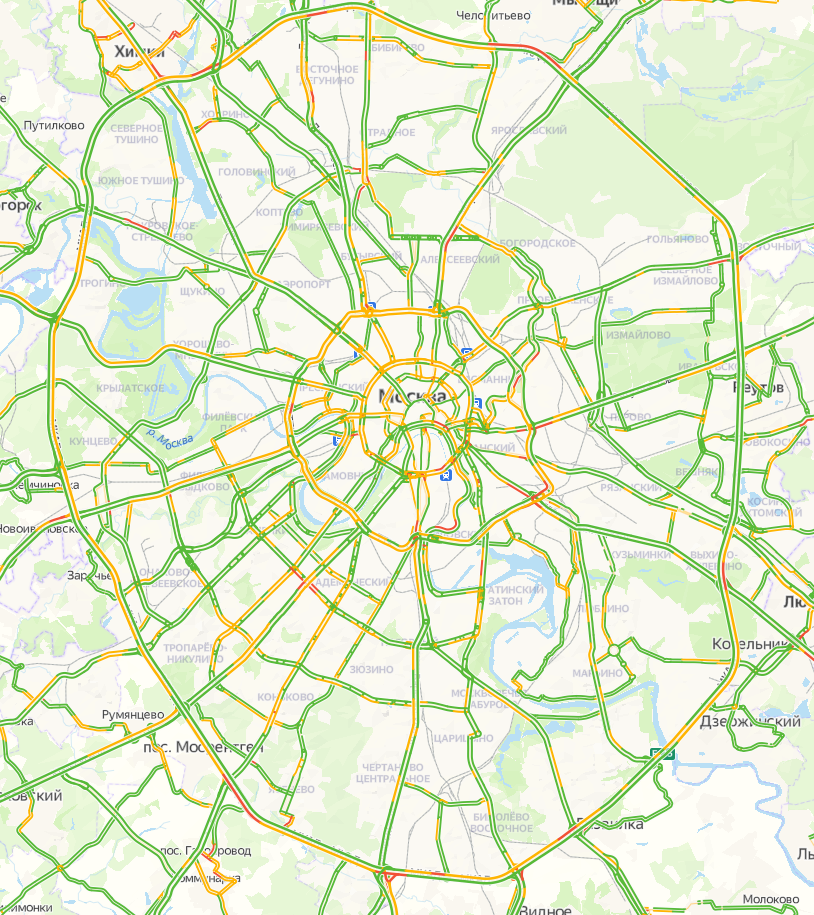
\includegraphics[width=0.5\linewidth]{YandexMap2.png}
        \caption{Типичные пробки по понедельникам в 18:15 на основе статистики сервиса «Яндекс-пробки» транспортной сети Москвы и МКАД, в частности по состоянию на 16.05.21.}
    \end{figure}
\end{frame}

\begin{frame}
    \frametitle{Мотивация к данной работе}
    \begin{itemize}
        \item Планы ЦОДД по управляемому въезду на МКАД,
        \item Микроскопические модели вычислительно тяжёлые,
        \item Макроскопическим моделям возможно не хватает точности;
    \end{itemize}

    Компромисс~--- рассматривать вместо движения каждого отдельного автомобильно-транспортного средства (АТС) движение их групп.
\end{frame}

\section{Математическая модель}
\begin{frame}[plain, noframenumbering]
    \begin{center}
        \Huge
        Математическая модель
    \end{center}
\end{frame}

\subsection{Транспортная сеть}
\begin{frame}
    \frametitle{Транспортная сеть}

    Транспортная сеть представляет собой связный ориентированный граф \(\mathbf{G} = (\mathbf{V}, \mathbf{E})\), где \(\mathbf{V}\) - множество вершин, \(\mathbf{E} = \{(i, j)\}\) - множество ветвей графа.

    Ограничения накладываемые на граф:
    \begin{itemize}
        \item \(\min(d(i)) = 1\),
        \item \(\max(d(i)) = 3\),
        \item \(\forall i: d(i) > 1 \rightarrow \exists j, l \in \mathbf{V} : (j, i), (i, l) \in \mathbf{E}\);
    \end{itemize}
\end{frame}

\subsection{Свойства группы АТС}
\begin{frame}
    \frametitle{Свойства группы АТС}
    Свойства группы АТС на ветви \((i, j): \mathbf{A}^t_k = \{\mathrm{Pos}_k, V_k, N_k\}:\)
    \begin{enumerate}
        \item \(\mathrm{Pos}_k\)~--- позиция начала группы относительно начала ветви на которой она расположена,
        \item \(V_k\)~--- скорость группы АТС,
        \item \(N_k\)~--- размер группы АТС из \(\mathbb{R}_{\geq 0} = \mathbb{R}_+\);
    \end{enumerate}

    Пусть теперь \(\mathbf{A}^t_{i,j} = \{\mathbf{A}^t_k\}\)~--- упорядоченное множество автомобильных групп на ветви \((i,j)\).

    \begin{block}{Состояние системы в момент времени \(t\)}
    \(\mathbf{A}^t = \{\mathbf{A}^t_{i,j}\} \cup \{A^t_{\text{out}, i, j}\}\)
    \end{block}
\end{frame}

\begin{frame}
    \frametitle{Расчёт характеристик группы АТС}
    \begin{enumerate}
      \item Скорость группы рассчитывается на основе плотности автомобилей на ветви автомагистрали и фундаментальной диаграммы поток-плотность.
      \item Длинна группы АТС считается линейно зависящей от ее скорости по формуле \(L = L_\text{avg} + a\cdot V\).
    \end{enumerate}
\end{frame}


\subsection{Процедура расчёта}
\begin{frame}
    \frametitle{Необходимые алгоритмы}
    \begin{itemize}
        \item Движение групп АТС по ветви,
        \item Объединение двух групп АТС,
        \item Перемещение групп АТС между ветвями,
        \item Расчёта потенциала трансфера между ветвями;
    \end{itemize}
\end{frame}

\begin{frame}
    \frametitle{Расчётный цикл}
    \begin{enumerate}
      \item Генерируем АТС всеми источниками в модели.
      \item Движение групп АТС на всех сегментах автомагистрали в порядке удалённости от конца магистрали.
      \item Очистка всех сегментов-стоков в модели от транспортных средств. Возврат к п.1.
    \end{enumerate}
\end{frame}

\section{Фундаментальная диаграмма потока}
\begin{frame}[plain, noframenumbering]
    \begin{center}
        \Huge
        Фундаментальная диаграмма потока
    \end{center}
\end{frame}

\begin{frame}
    \frametitle{Данные дорожных датчиков}
    \begin{figure}[ht]
        \begin{center}
            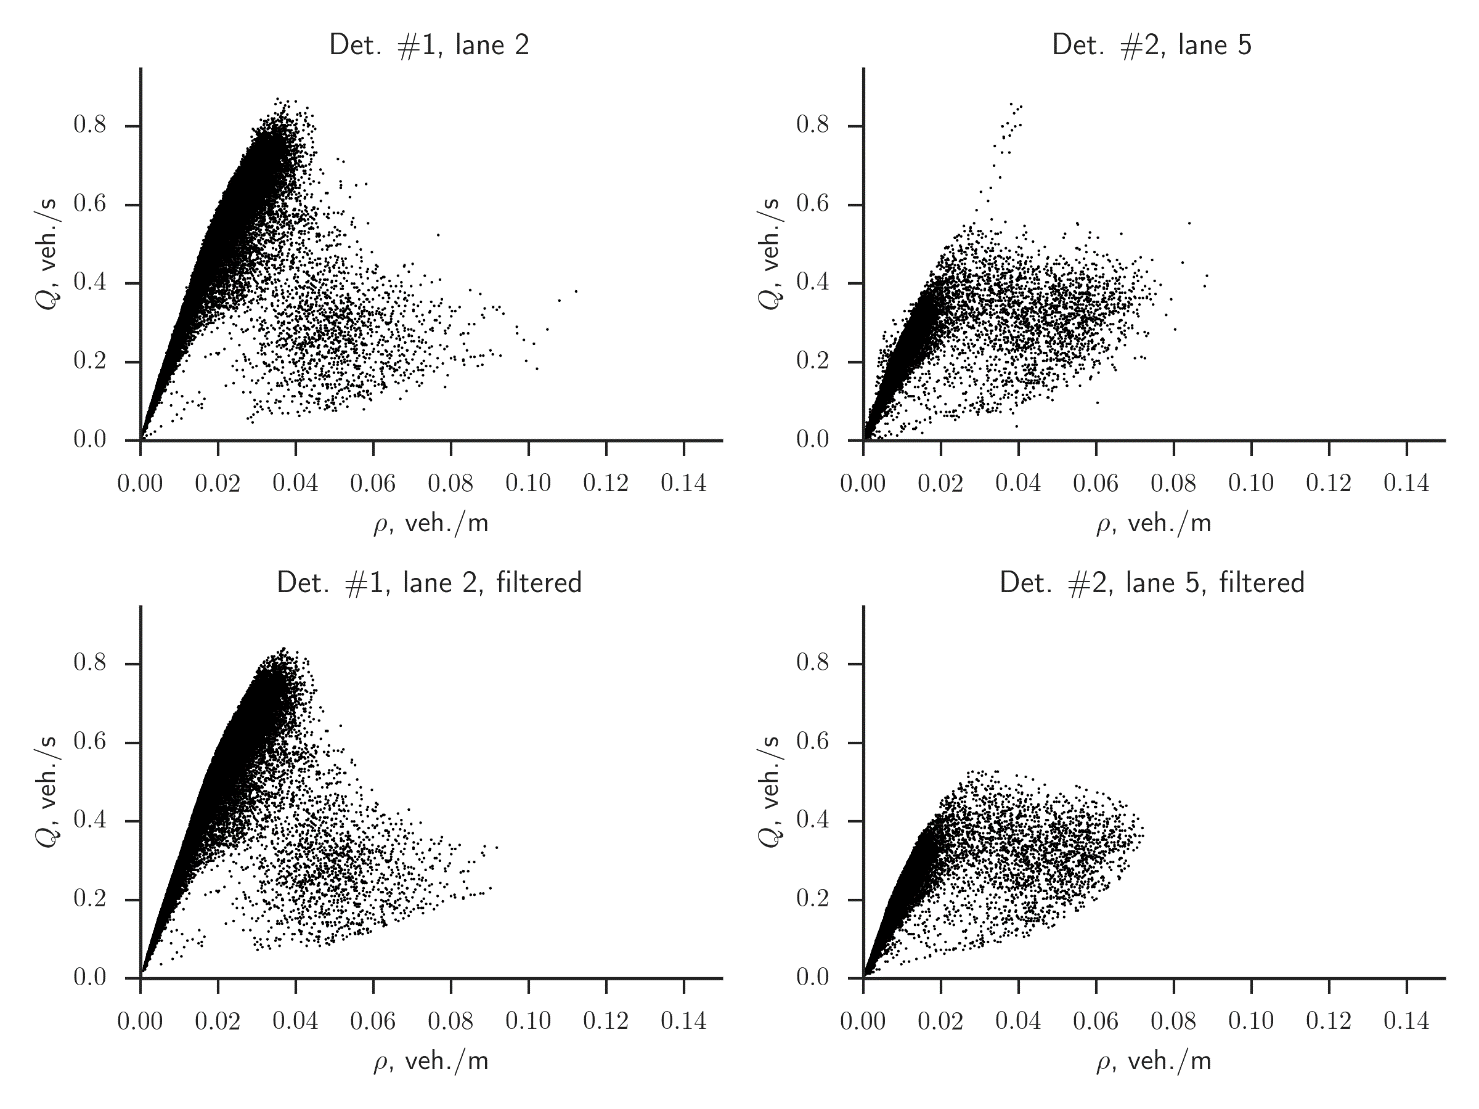
\includegraphics[width=1\linewidth]{detectors_data_alpha.png}
            \caption{Экспериментальные данные с двух детекторов, установленных на различных полосах МКАД --- замеренные интенсивности транспортного потока \(Q(\rho)\)[АТС/с] при различной плотности [АТС/м]. Данные представлены за 2012 г. В количестве 288 измерений за день. Сверху исходные данные, снизу отфильтрованные с использованием алгоритма построения выпуклых оболочек.}
        \end{center}
    \end{figure}
\end{frame}

\begin{frame}
    \frametitle{Три фазы Кернера}
    \begin{enumerate}
      \item Свободный поток \(Q(\rho) = \alpha_2\rho^2 + \alpha_1\rho,\ 0\leq\rho\leq\rho_1\),
      \item Синхронизованный поток \(Q(\rho) = \beta_2\rho^2 + \beta_1\rho + \beta_0,\ \rho_1\leq\rho\leq\rho_2\),
      \item Заторный поток \(Q(\rho) = c_*(\rho_*-\rho),\ \rho_1\leq\rho\leq\rho_*\);
    \end{enumerate}
    
    Kerner, B. S. Introduction to modern traffic flow theory and control [Текст]. Т. 700 / B. S. Kerner. — Springer, 2009.
\end{frame}

\begin{frame}
    \frametitle{Пример фундаментальных диаграмм}
    \begin{figure}[ht]
        \begin{center}
            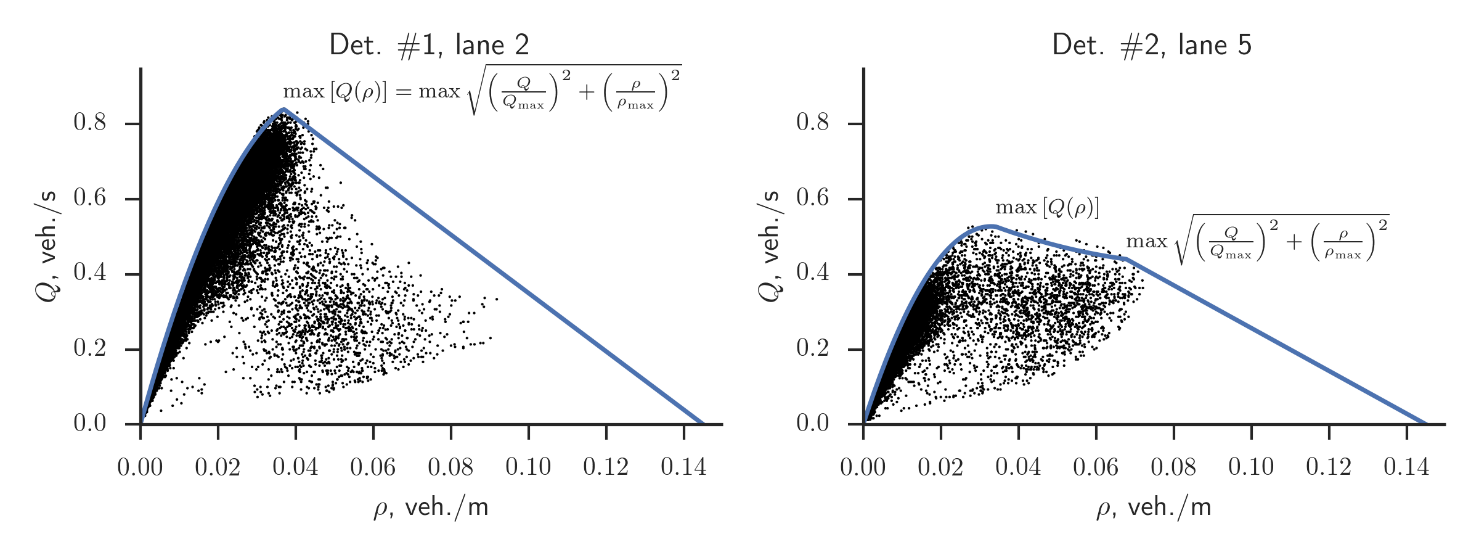
\includegraphics[width=1\linewidth]{Q_result.png}
            \caption{Фундаментальные диаграммы для двух разных участков МКАД. Слева для данных со второй полосы (детектор № 1), справа с пятой полосы (детектор №2)}
        \end{center}
    \end{figure}

\end{frame}

\begin{frame}
    \frametitle{Расчет скорости волны торможения}
    \begin{figure}[ht]
        \begin{center}
            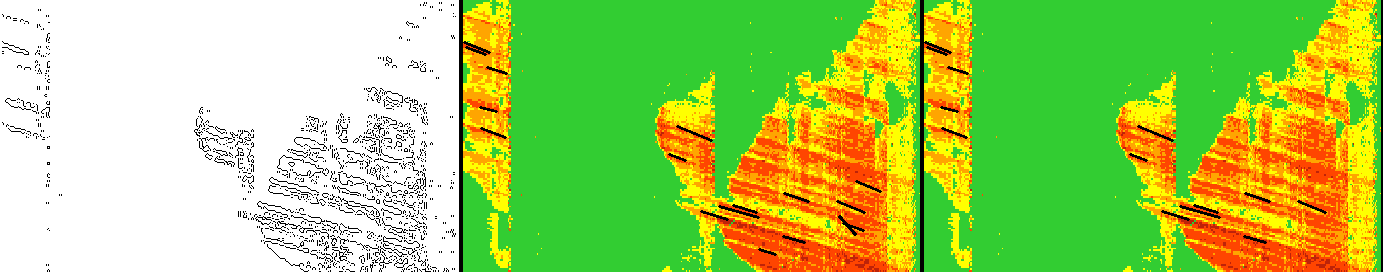
\includegraphics[width=1\linewidth]{c_end.png}
            \caption{Нахождение значений скорости волн торможения на пространственно-временной структуре значений скорости транспортного потока на внешней стороне МКАД}
        \end{center}
    \end{figure}

    Итоговая скорость волны торможения равна \(-15,8\) км/ч.
\end{frame}


\section{Комплексирование данных}
\subsection{Комплексирование данных}
\begin{frame}[plain, noframenumbering]
    \begin{center}
        \Huge
        Комплексирование данных
    \end{center}
\end{frame}

\subsection{Необходимость комплексирования данных}
\begin{frame}
    \frametitle{Необходимость комплексирования данных}
    \begin{enumerate}
      \item Дорожные датчики относительно точны, но не покрывают всю транспортную сеть.
      \item GPS-треки имеют низкую точность, но покрывают большой объём транспортной сети.
    \end{enumerate}
\end{frame}

\subsection{Функциональная зависимость реального числа АТС от трекового}
\begin{frame}
    \frametitle{Функциональная зависимость реального числа АТС от трекового}
    \centering
    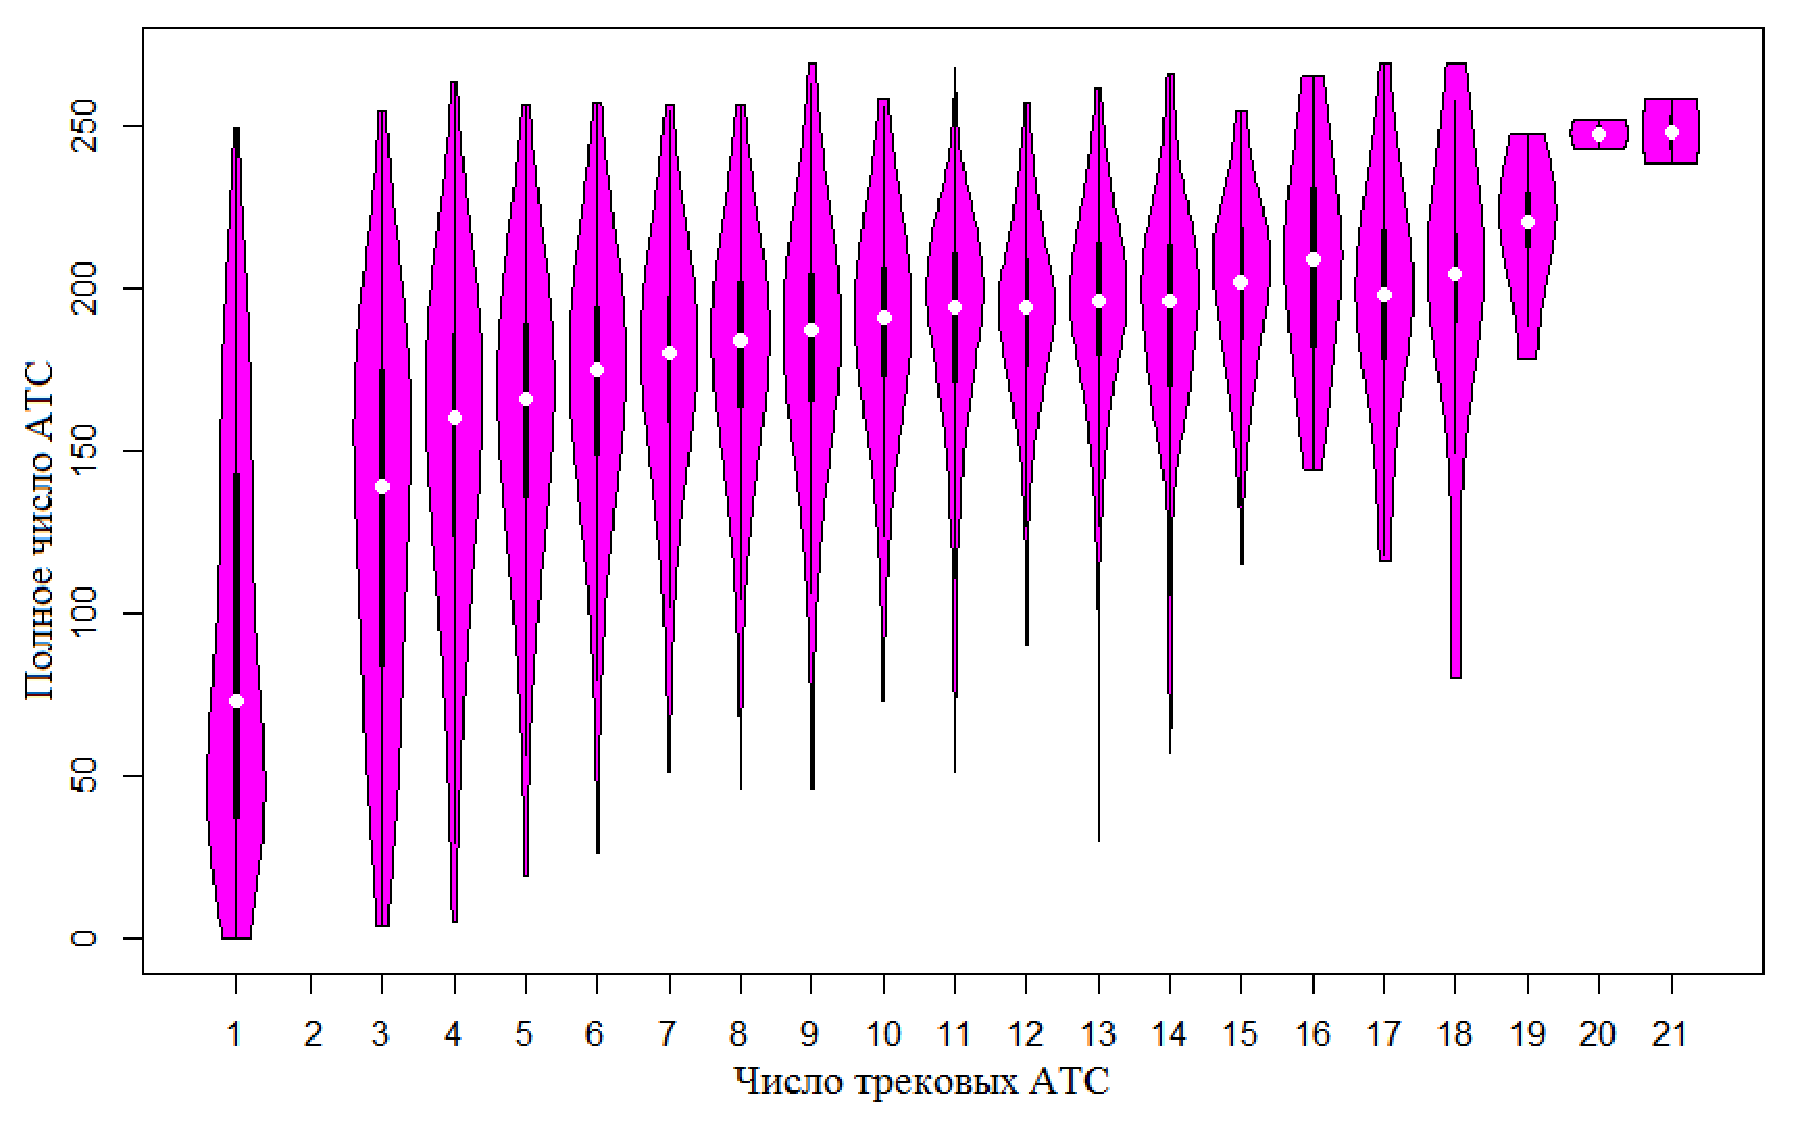
\includegraphics[width=1\linewidth]{Vioplot_Detector-Yandex.eps}
    \begin{equation*}
        \begin{split}
            & N_{\text{real}} = a_0 + a_1N_{\text{track}} + a_2\log\left({N_{\text{track}}}\right) + a_3V + a_4N_{\text{track}}/V
        \end{split}
    \end{equation*}
\end{frame}

\subsection{Преобразование скорости}
\begin{frame}
    \frametitle{Преобразование скорости}
\vspace{-4mm}
\begin{equation*}
    V_{\text{est}} = 12.34 + 0.639V_{\text{track}}
    \label{eq::speed_transform}
\end{equation*}

\vspace{-2mm}
\begin{table}[!ht]
    \centering
    \begin{tabular}{|c|c|c|}
         \hline
         & $V_{\text{est}}$ & $V_{\text{track}}$ \\
         \hline
         Среднеквадратичная ошибка & \textbf{0.03} & 0.042 \\
         \hline
    \end{tabular}
\end{table}
\vspace{-4mm}

    \begin{figure}[!ht]
    \subfloat{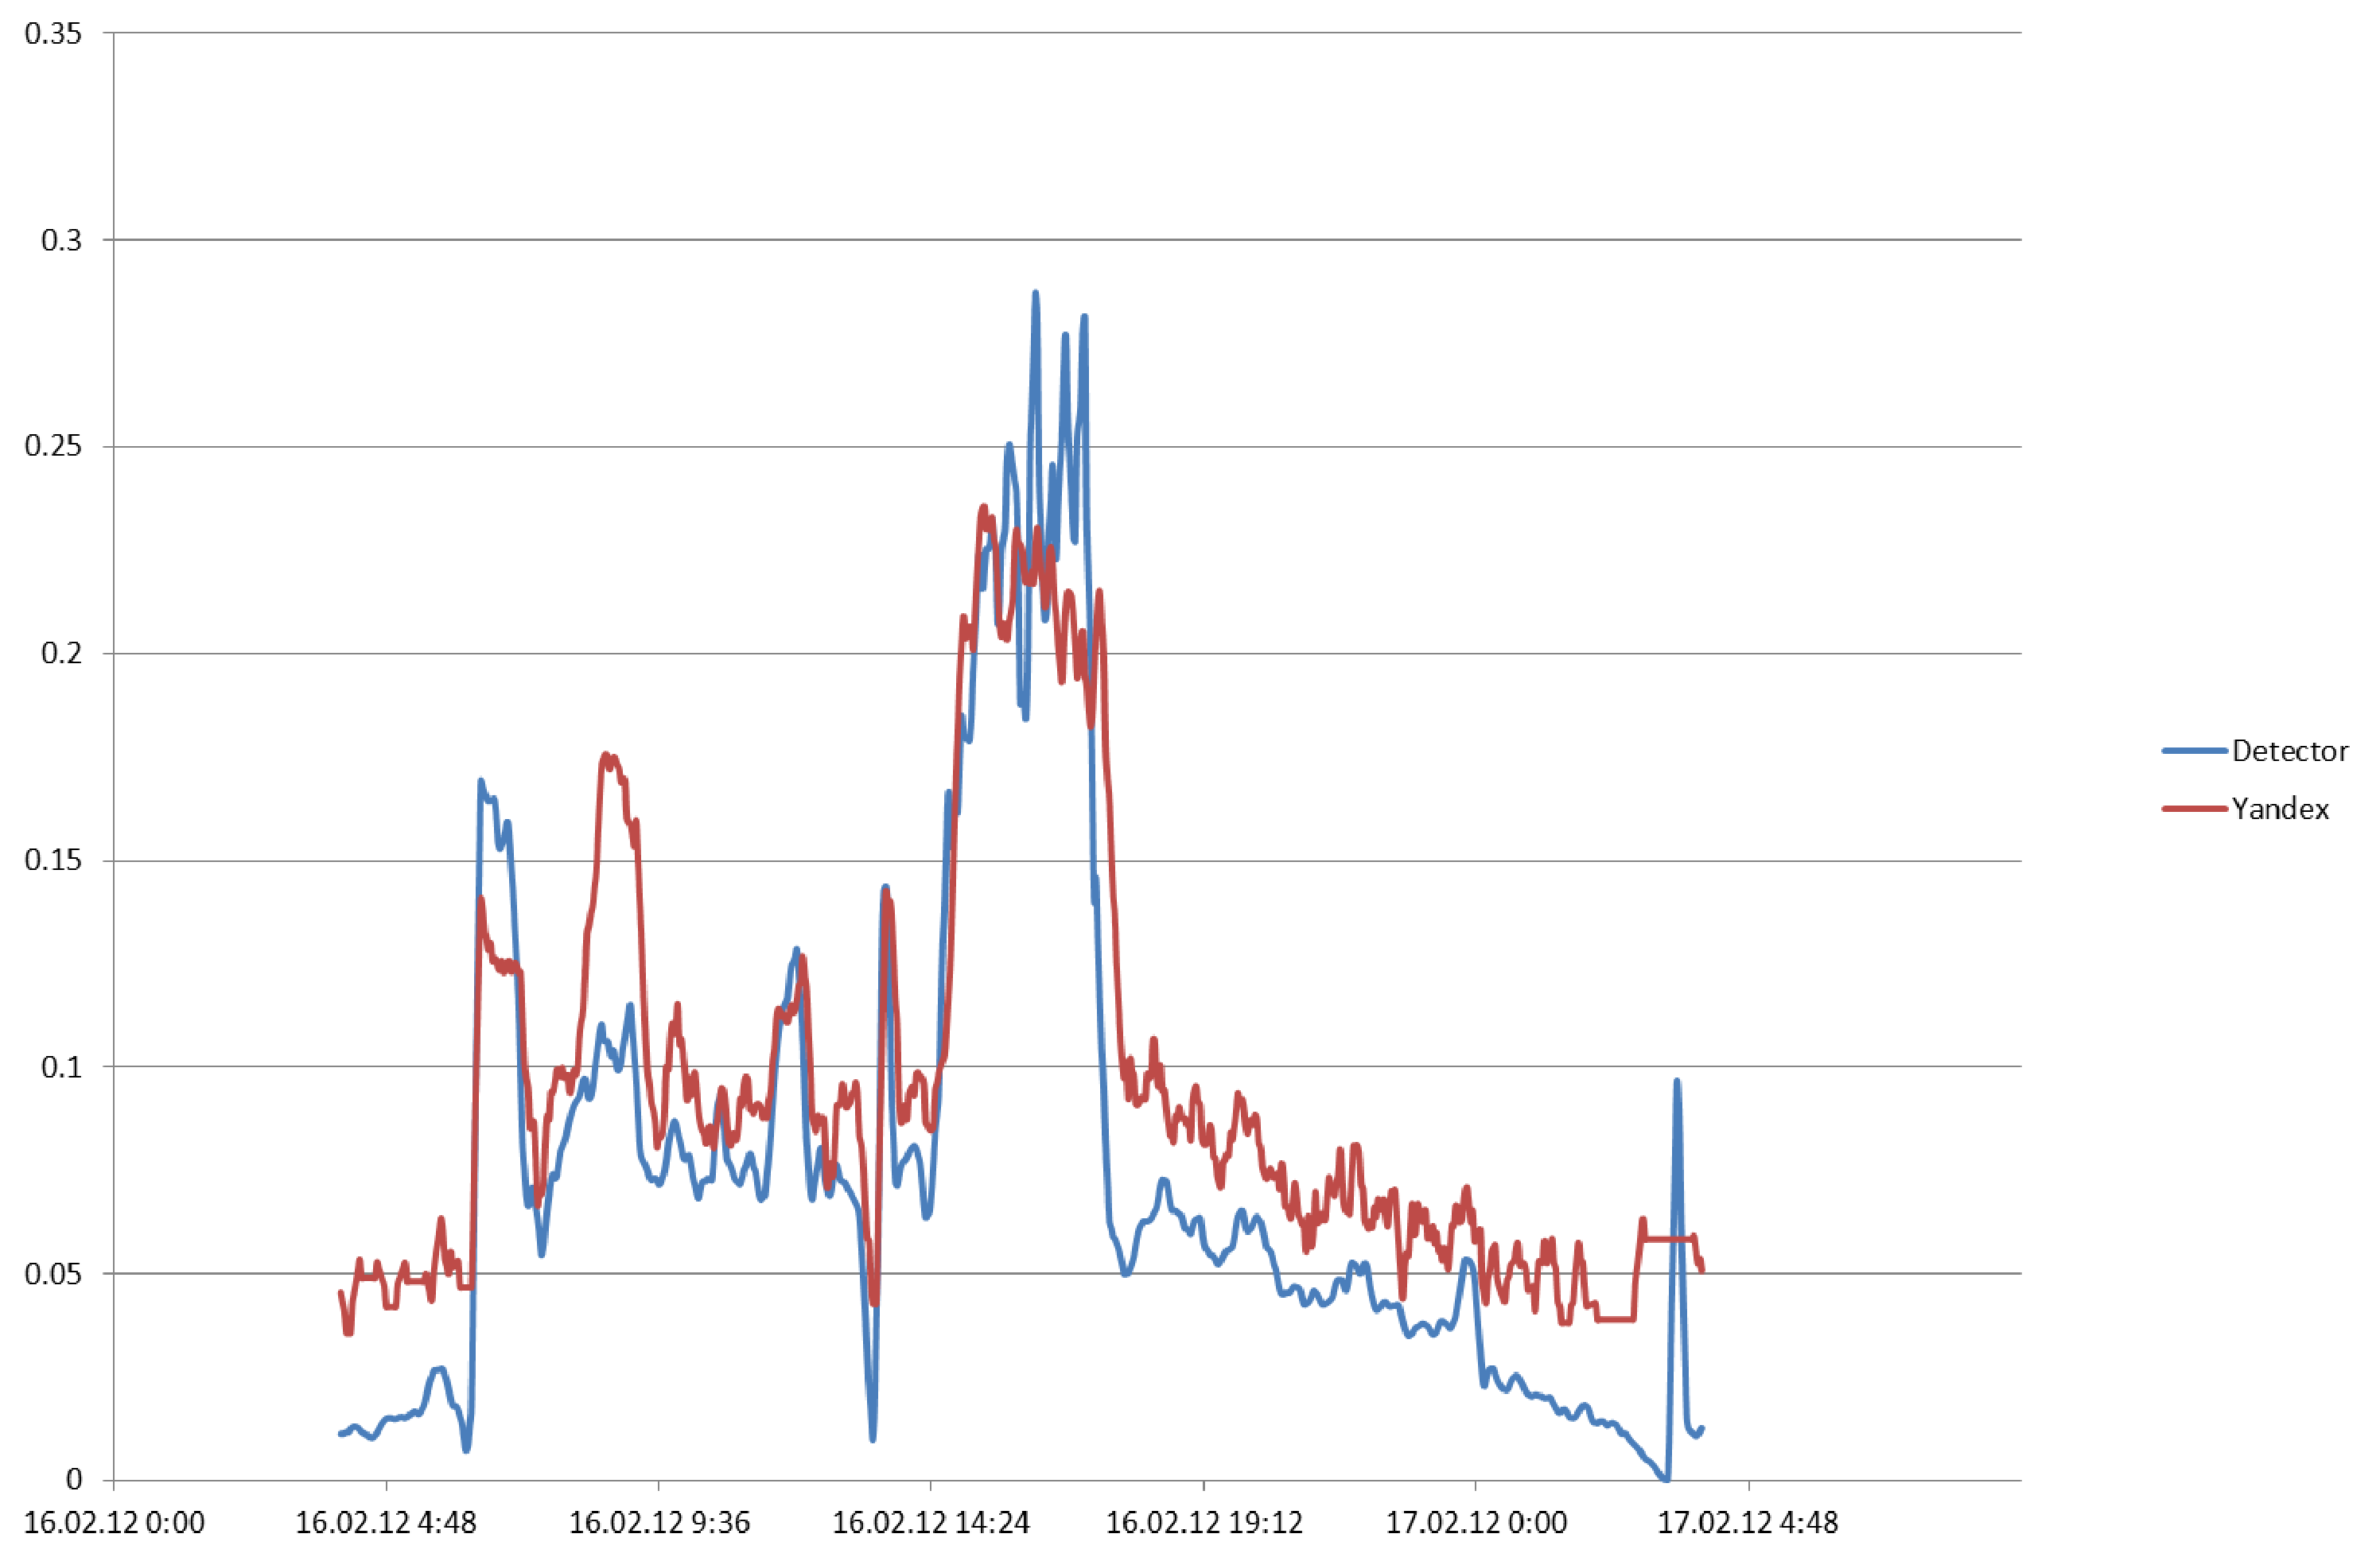
\includegraphics[width=0.45\linewidth]{With_V.eps}}
    \subfloat{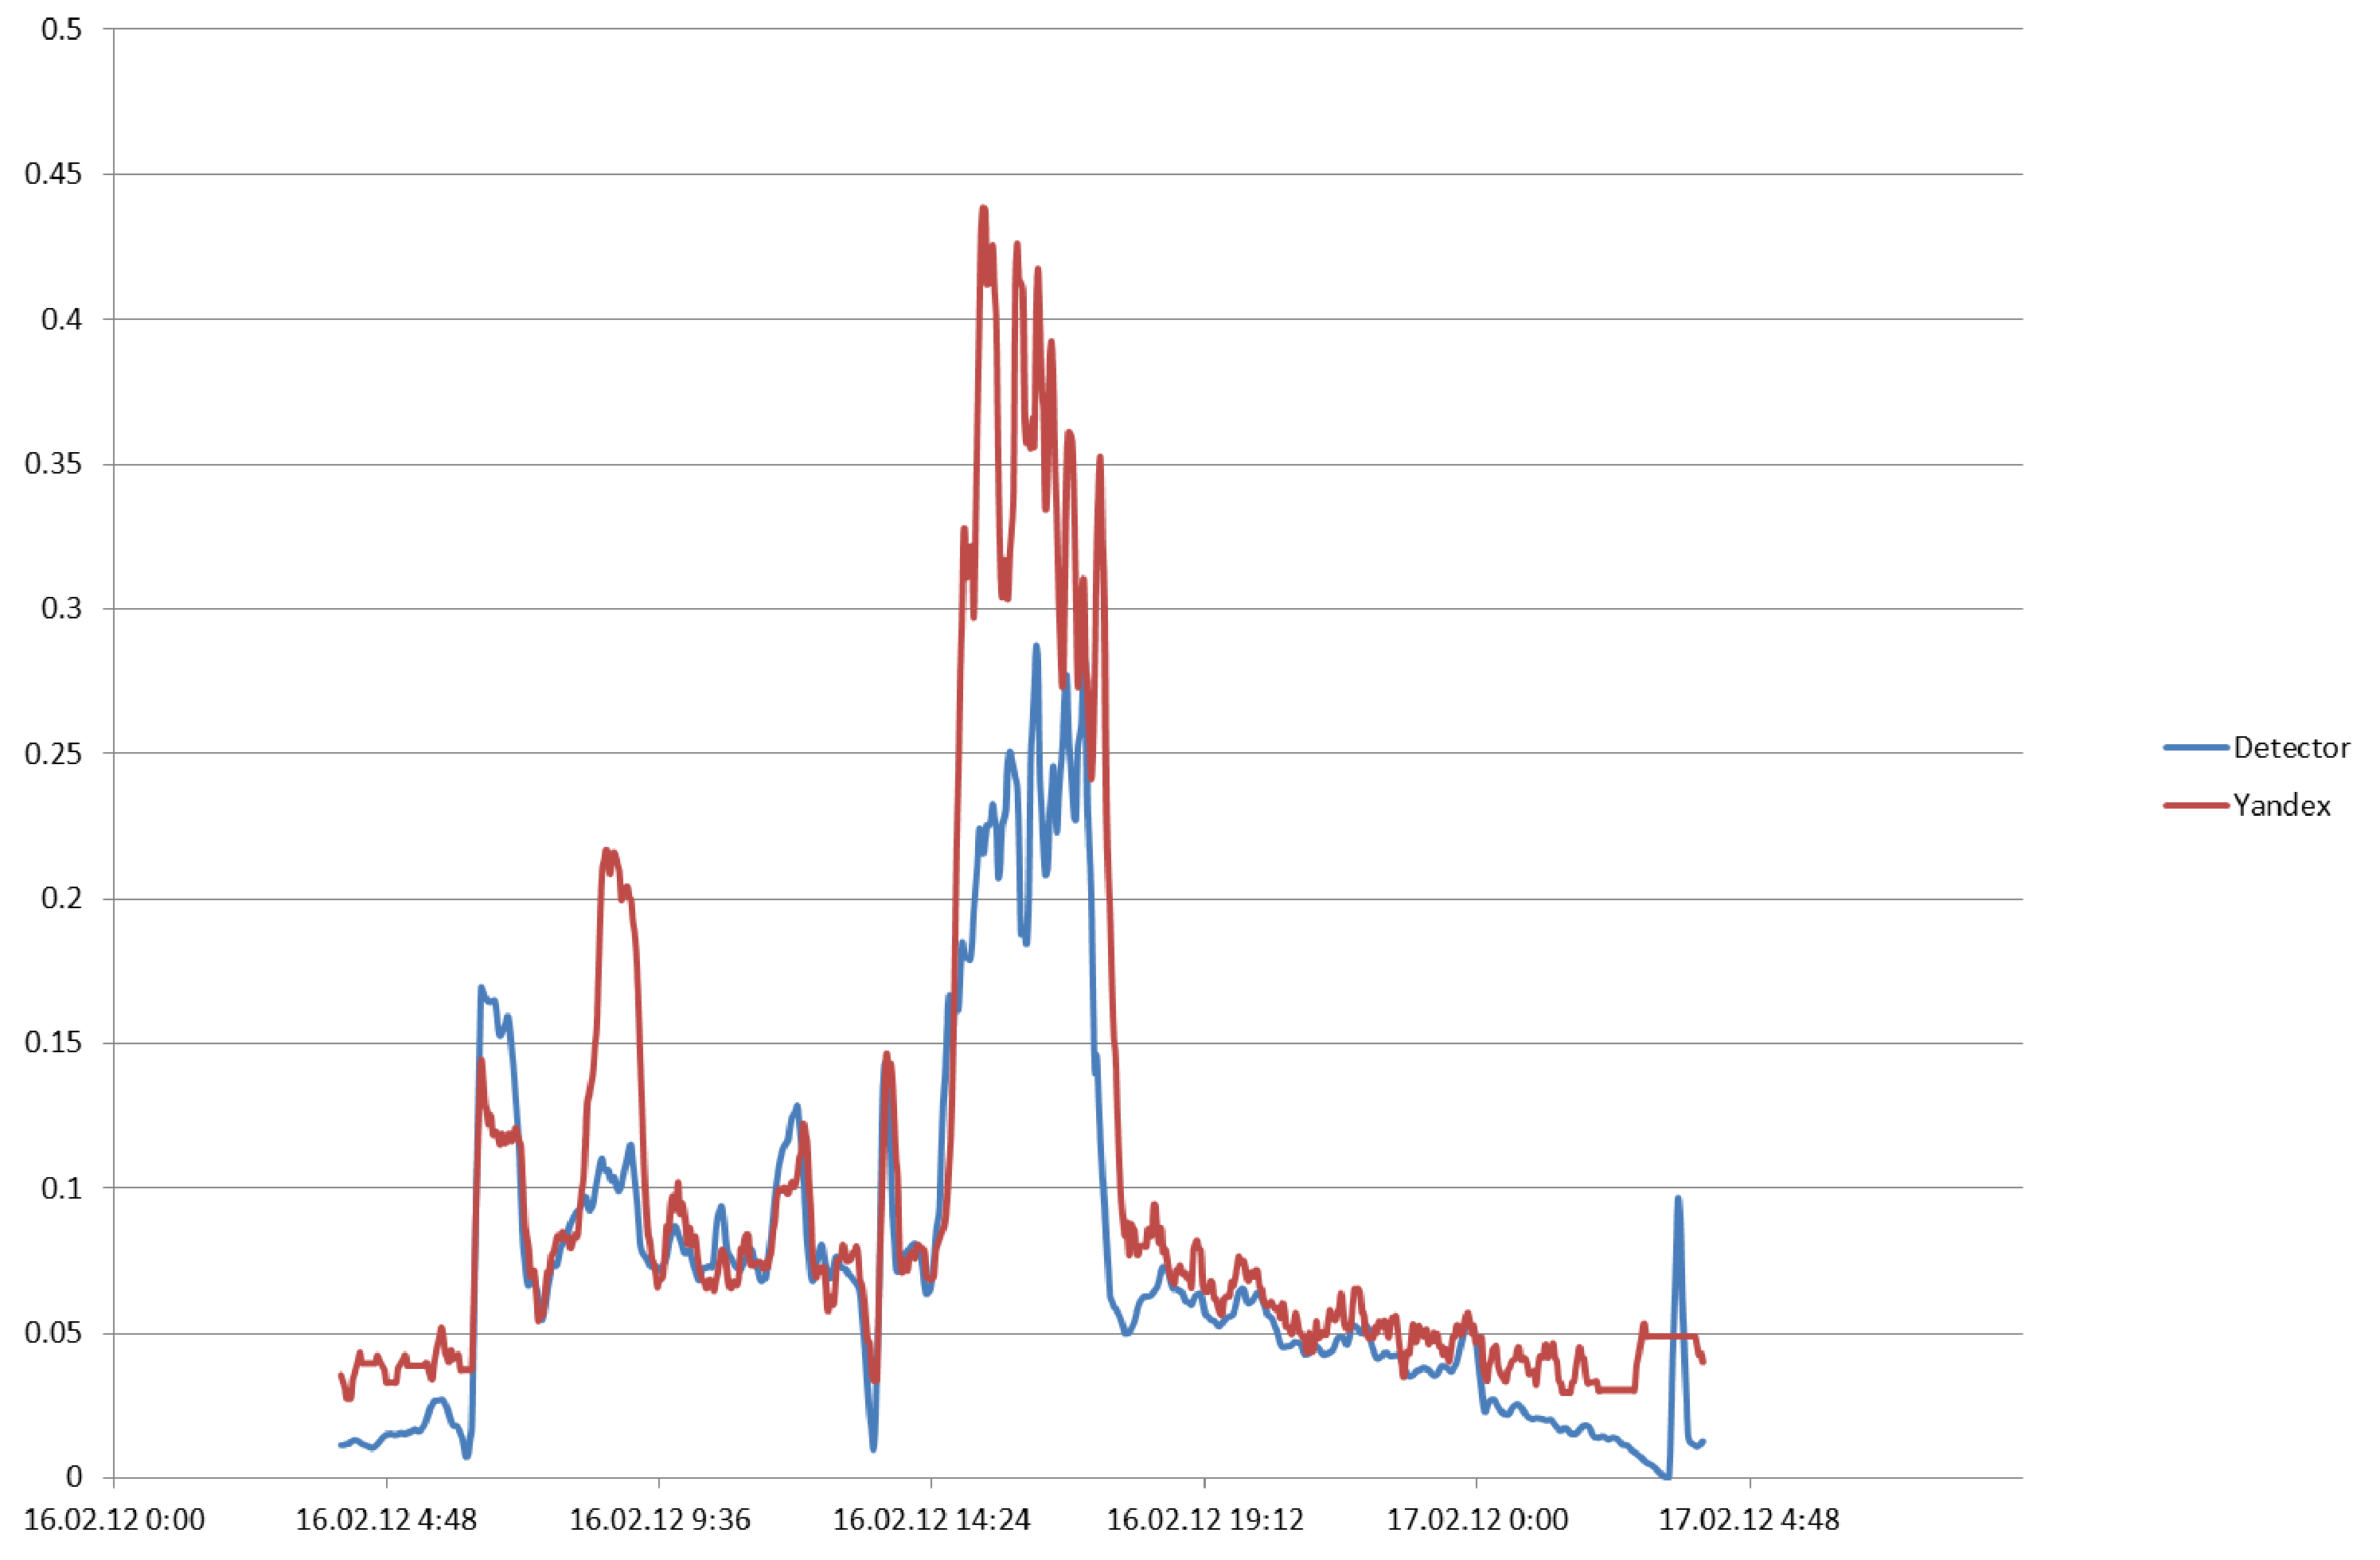
\includegraphics[width=0.45\linewidth]{Without_V.eps}}
    \caption{Восстановленные значения плотности АТС с (слева) и без (справа) преобразования скорости}
    \end{figure}
\end{frame}


\section{Вычислительные эксперименты}
\subsection{Проверка работоспособности модели}
\begin{frame}[plain, noframenumbering]
    \begin{center}
        \Huge
        Проверка работоспособности модели
    \end{center}
\end{frame}

\begin{frame}
    \frametitle{Простая дорога}
  \hfil\hfil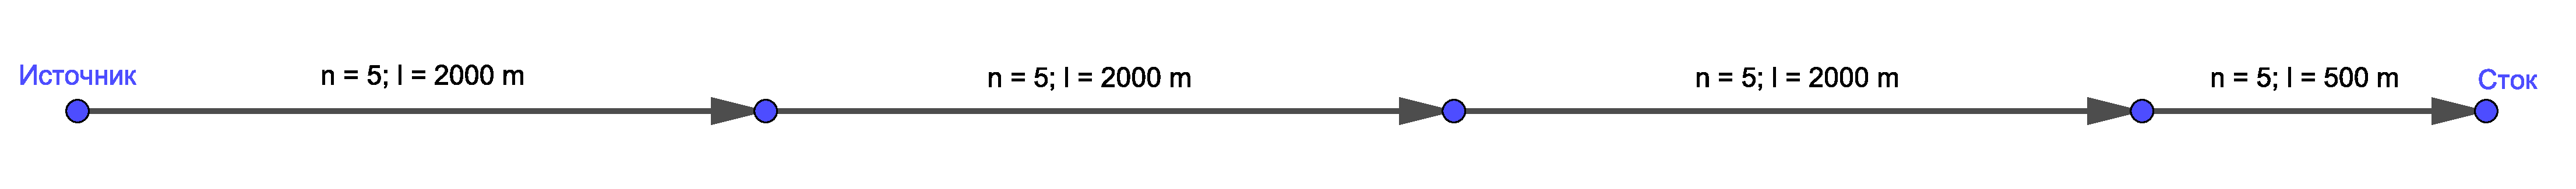
\includegraphics[width=1.0\linewidth]{scheme_simple_3block_road.eps}\newline
  \vfil
  \hfil\hfil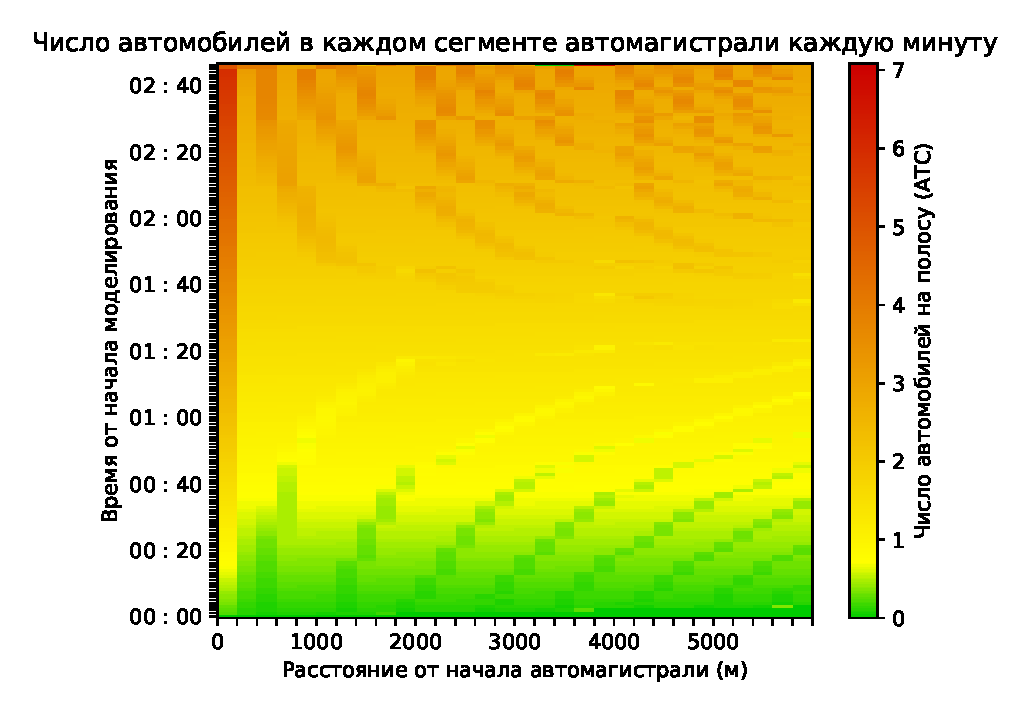
\includegraphics[width=0.5\linewidth]{simple_3_block_road.eps}\hfil\hfil
    \begin{minipage}[b][0.5\textheight][c]{.45\linewidth}
    Простая дорога без перекрестков с линейно нарастающим вплоть до 150 АТС/мин потоком.
    \end{minipage}\newline
\end{frame}

\begin{frame}
    \frametitle{Дорога с сужением, синусоидальный поток}
  \hfil\hfil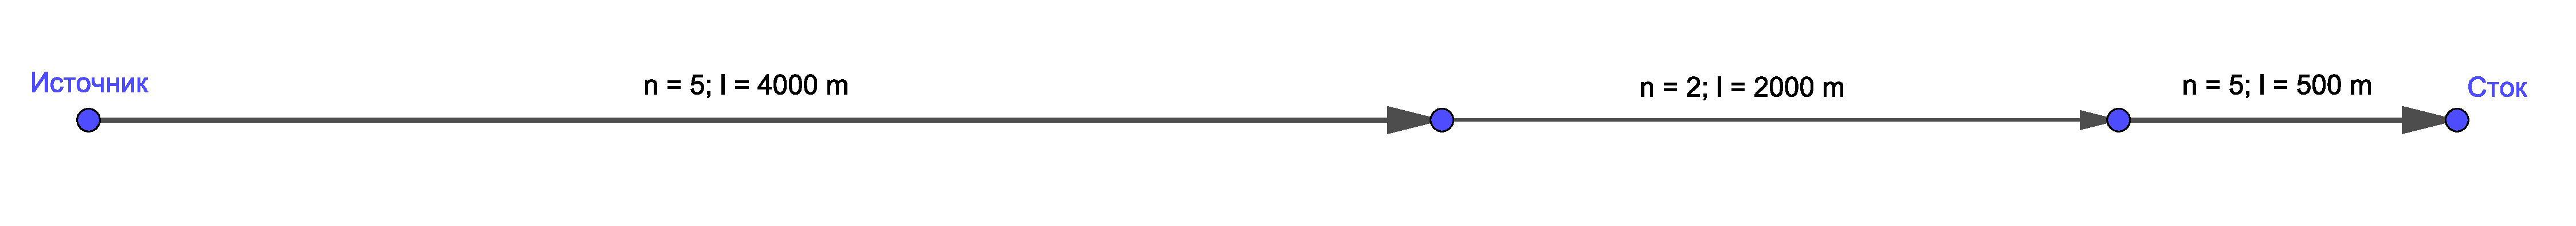
\includegraphics[width=1.0\linewidth]{scheme_jammed_sin_wave.eps}\newline
  \vfil
  \hfil\hfil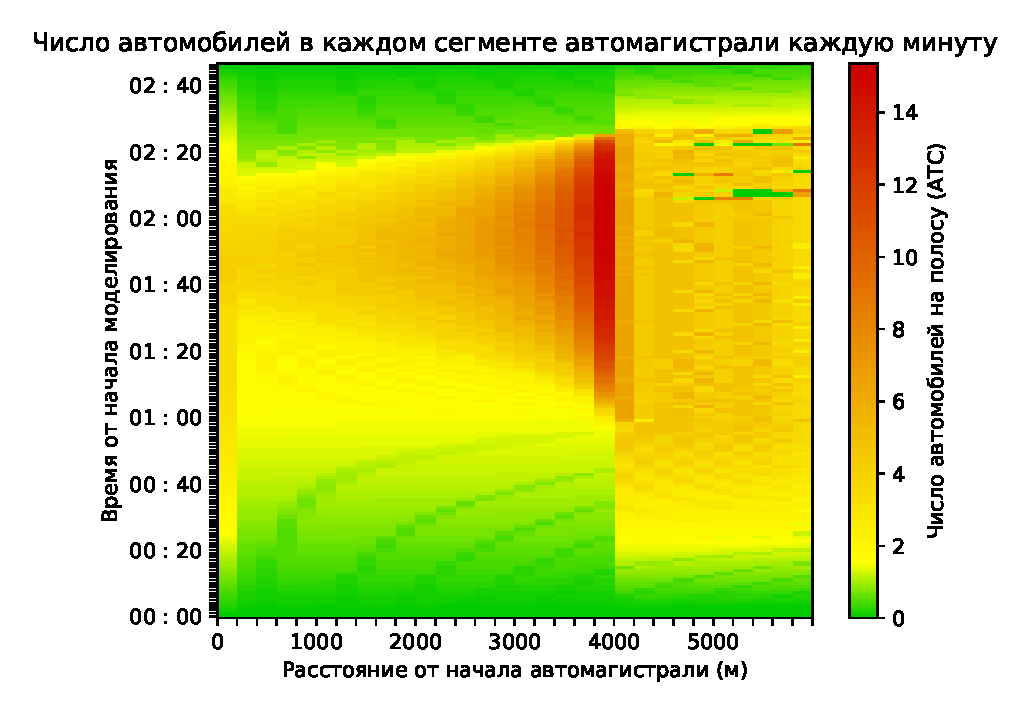
\includegraphics[width=0.5\linewidth]{jammed_5-2_3block_road_sin_wave}\hfil\hfil
    \begin{minipage}[b][0.5\textheight][c]{.45\linewidth}
    Пятиполосная дорога с сужением до двух полос. Входной поток~--- синусоида с периодом равным времени моделирования и амплитудой 85 АТС/мин.
    \end{minipage}\newline
\end{frame}

\begin{frame}
    \frametitle{Дорога с пропадающим сужением}
  \hfil\hfil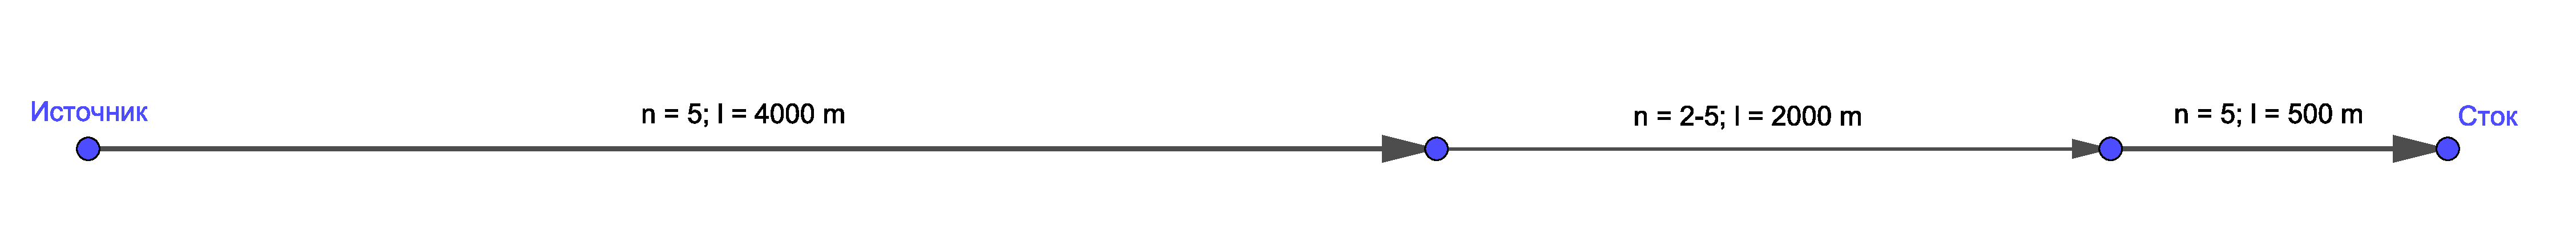
\includegraphics[width=1.0\linewidth]{scheme_jammed_with_unjam.eps}\newline
  \vfil
  \hfil\hfil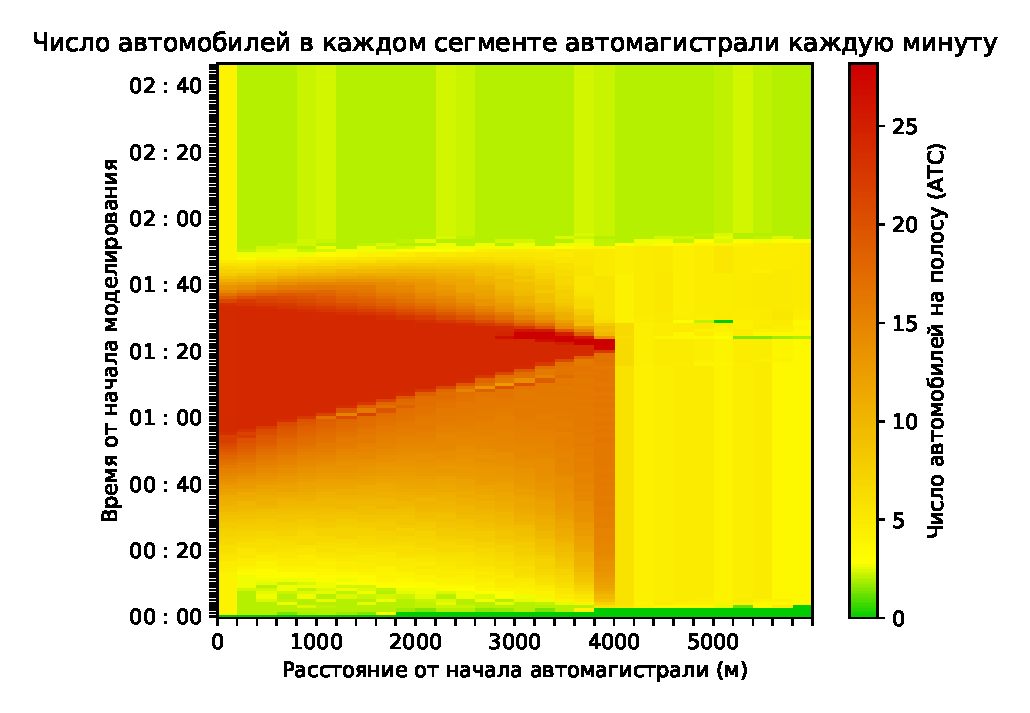
\includegraphics[width=0.5\linewidth]{jammed_5-2_3block_road_with_unjam.eps}\hfil\hfil
    \begin{minipage}[b][0.5\textheight][c]{.45\linewidth}
    Пятиполосная дороге без перекрестков с пропадающим сужением до двух полос. Входной поток 100 АТС/мин.
    \end{minipage}\newline
\end{frame}

\begin{frame}
    \frametitle{Съезд}
  \hfil\hfil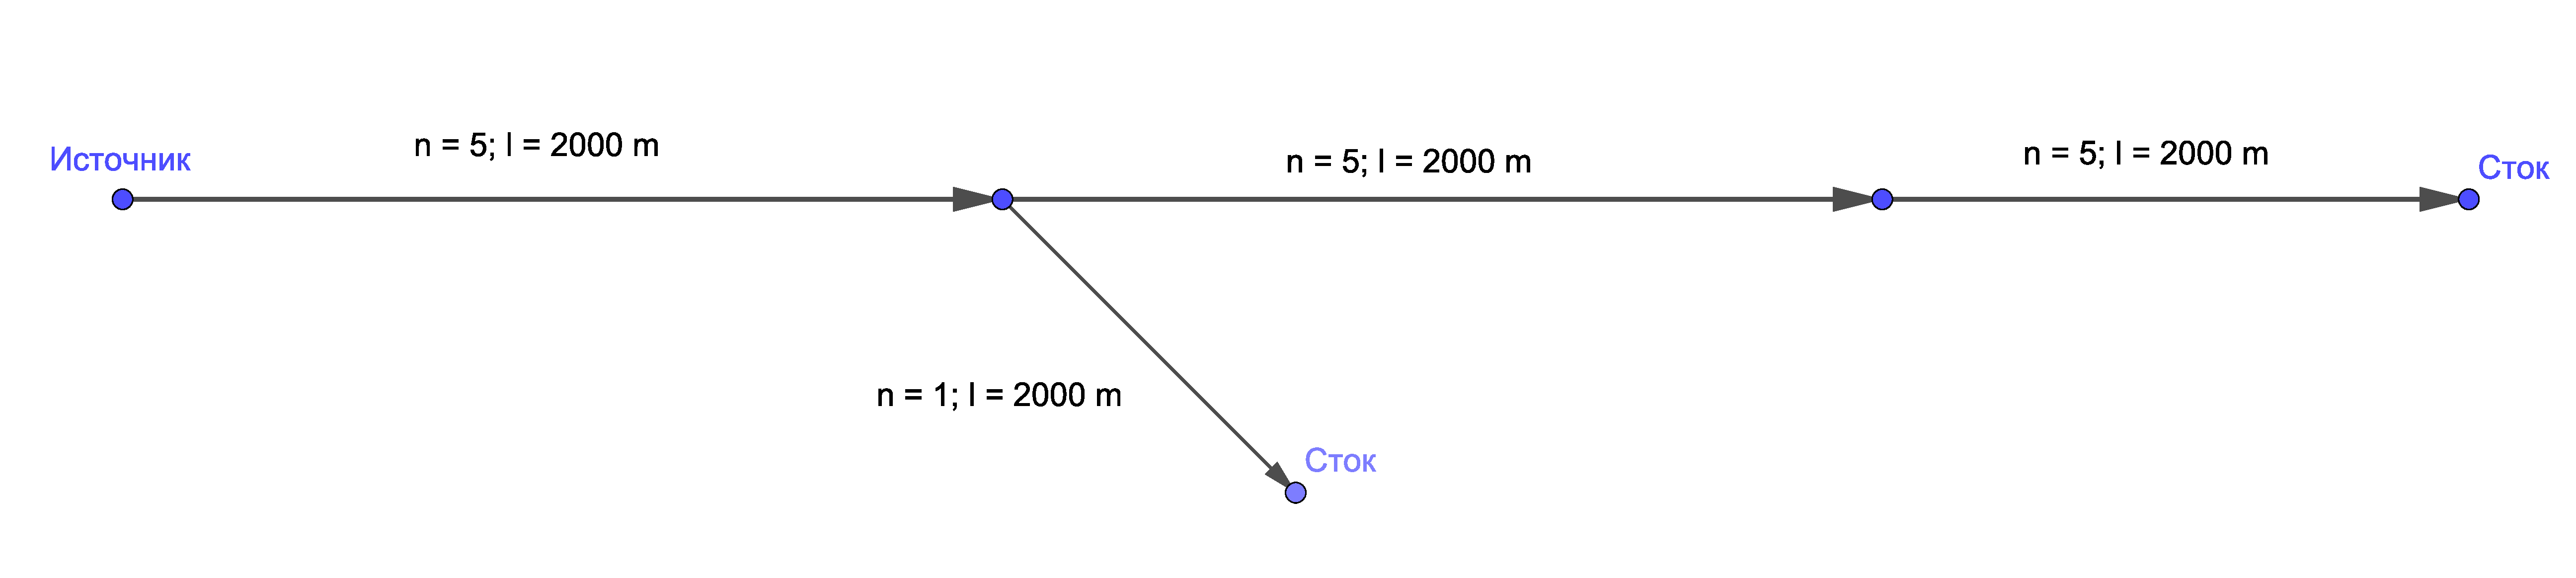
\includegraphics[width=1.0\linewidth]{scheme_jammed_crossroad_exit.eps}\newline
  \vfil
  \hfil\hfil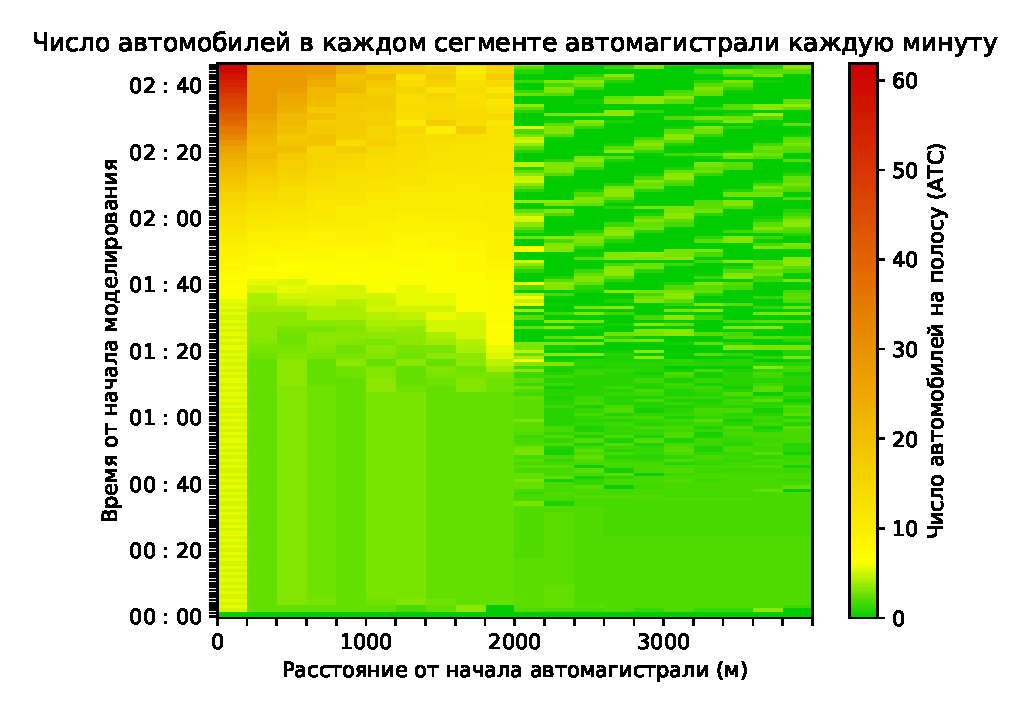
\includegraphics[width=0.5\linewidth]{jamming_crossroad_exit_5_1.eps}\hfil\hfil
    \begin{minipage}[b][0.5\textheight][c]{.45\linewidth}
    Пятиполосная дорога со съездом. Поток на автомагистрали 65 АТС/мин с линейно нарастающей долей съезжающих автомобилей с 20\% до 60\%.
    \end{minipage}\newline
\end{frame}

\begin{frame}
    \frametitle{Въезд}
  \hfil\hfil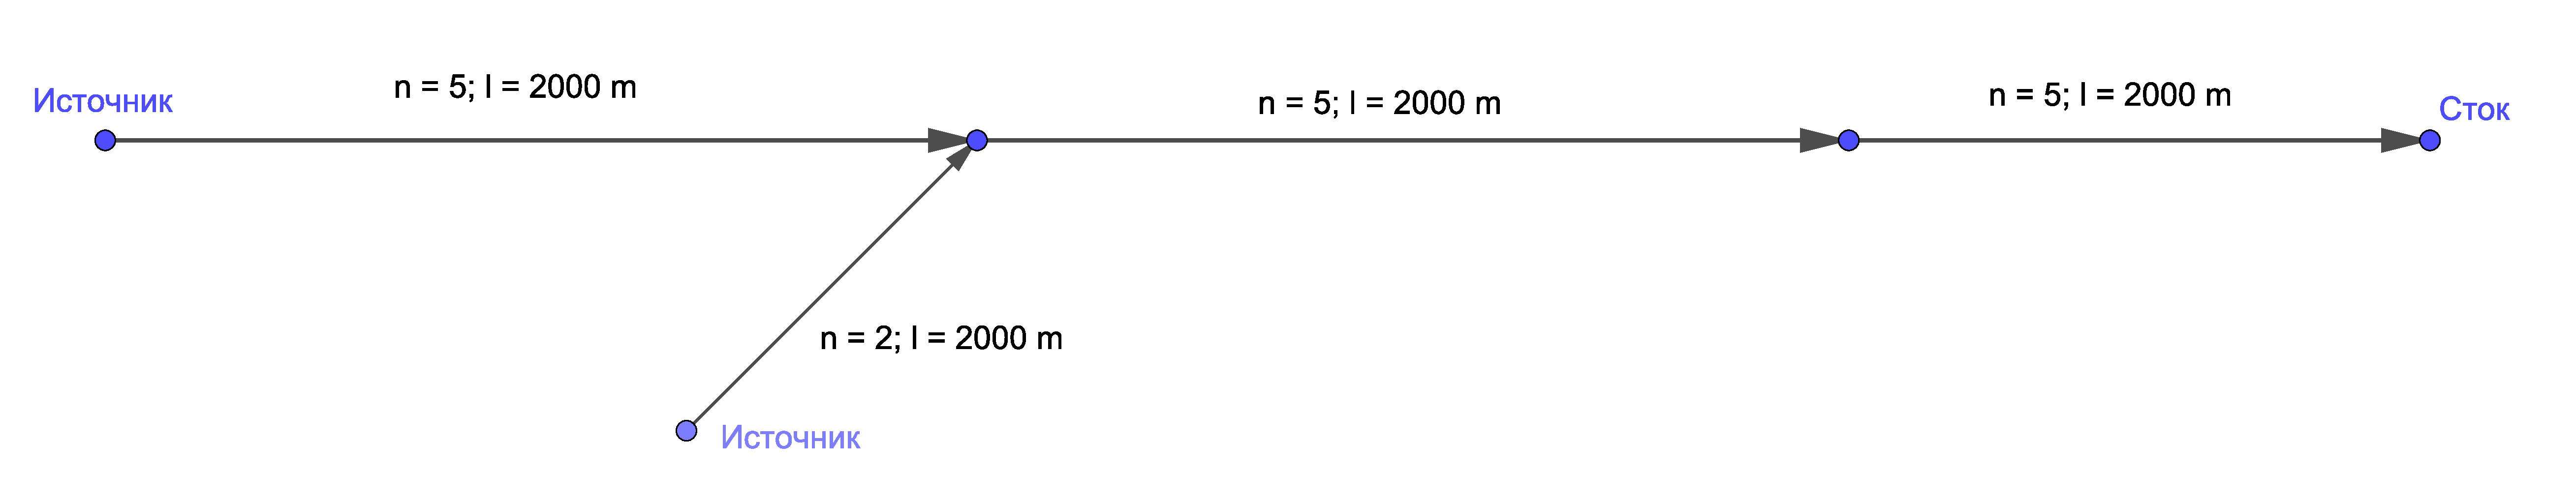
\includegraphics[width=1.0\linewidth]{scheme_jammed_crossroad_enter.eps}\newline
  \vfil
  \hfil\hfil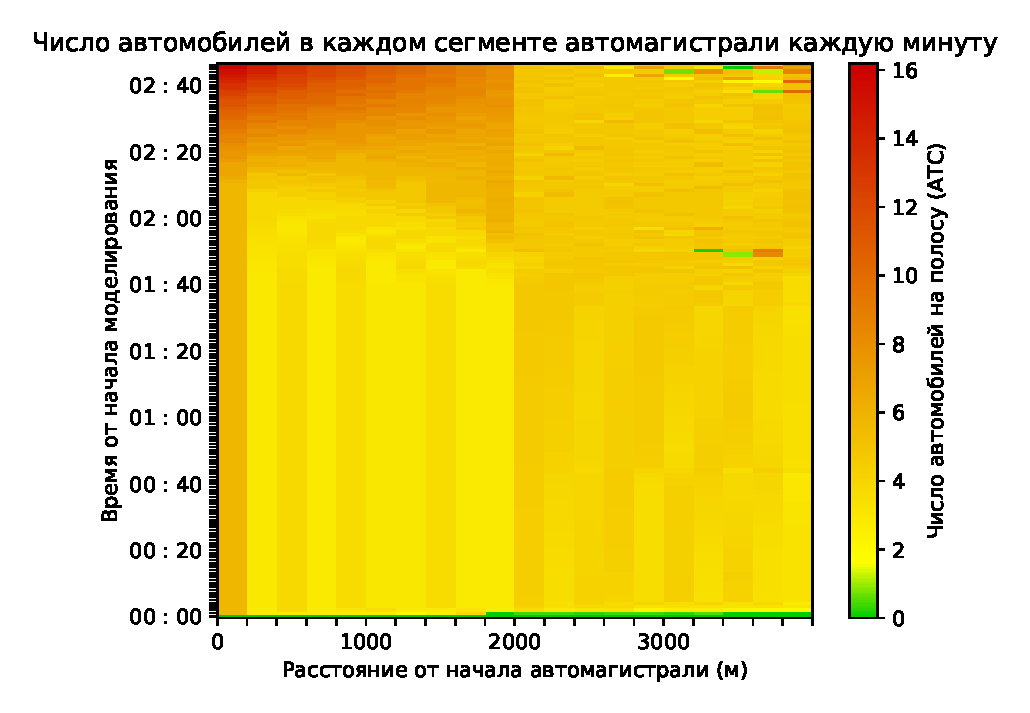
\includegraphics[width=0.5\linewidth]{jamming_crossroad_enter_5_2.eps}\hfil\hfil
    \begin{minipage}[b][0.5\textheight][c]{.45\linewidth}
    Пятиполосная дорога с въездом. Поток на автомагистрали 140 АТС/мин, поток на въезде линейно растет с 20 до 50 АТС/мин.
    \end{minipage}\newline
\end{frame}

\begin{frame}
    \frametitle{Прямая дорога между дорожными датчиками}
    \begin{figure}[h]
        \centering
        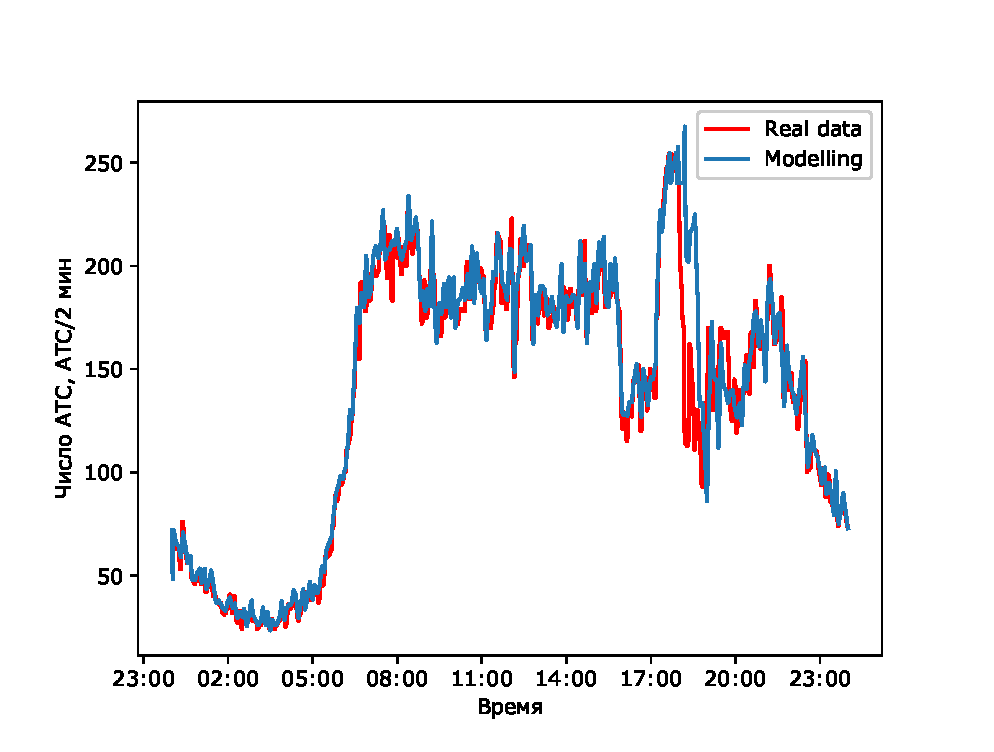
\includegraphics[width=0.6\linewidth]{MCAR_simple_test.eps}
        \caption{График полученного с помощью модели числа съехавших АТС (красная линия) в сравнении с числом съехавших АТС зафиксированных дорожным датчиком (синяя линия) за один день. Среднеквадратичная ошибка $S = 18.4$.}
    \end{figure}
\end{frame}

\begin{frame}
    \frametitle{Прямая дорога между дорожными датчиками. Перекрытая полоса}
    \begin{figure}[ht]
        \centering
        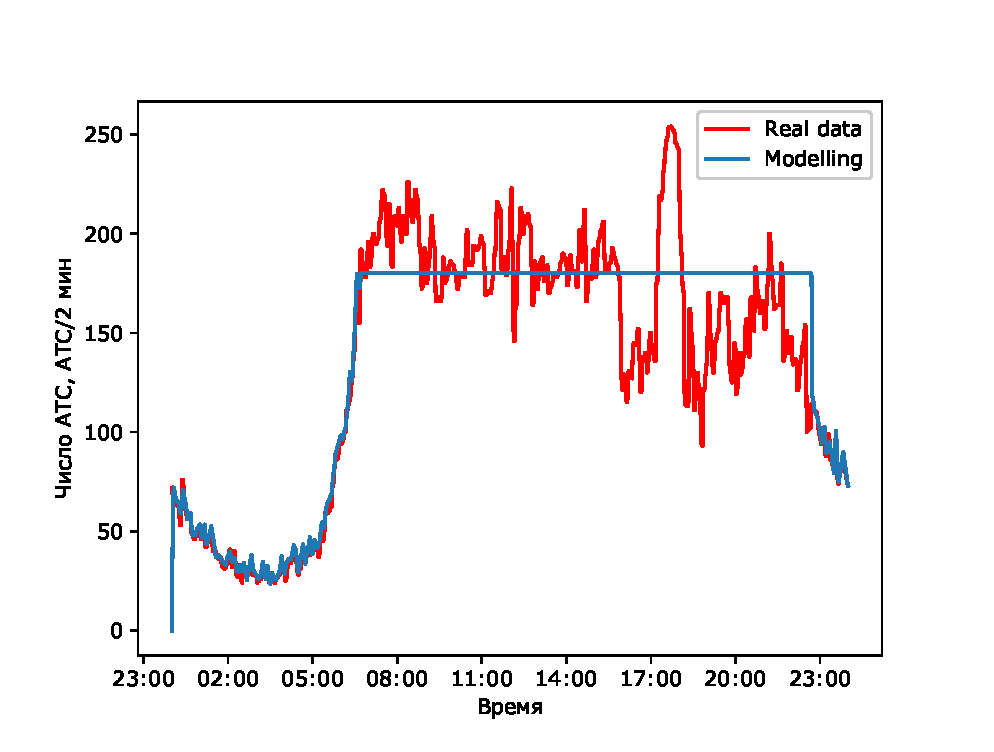
\includegraphics[width=0.6\linewidth]{MCAR_minus_line.eps}
        \caption{График полученного с помощью модели числа съехавших АТС (красная линия) в сравнении с числом съехавших АТС зафиксированных дорожным датчиком (синяя линия) за один день с перекрытием полосы.}
    \end{figure}
\end{frame}



\subsection{Моделирование МКАД}
\begin{frame}[plain, noframenumbering]
    \begin{center}
        \Huge
        Моделирование МКАД
    \end{center}
\end{frame}

\begin{frame}
    \frametitle{Дорожный датчик на въезде}
    \begin{figure}[ht]
    \centering
    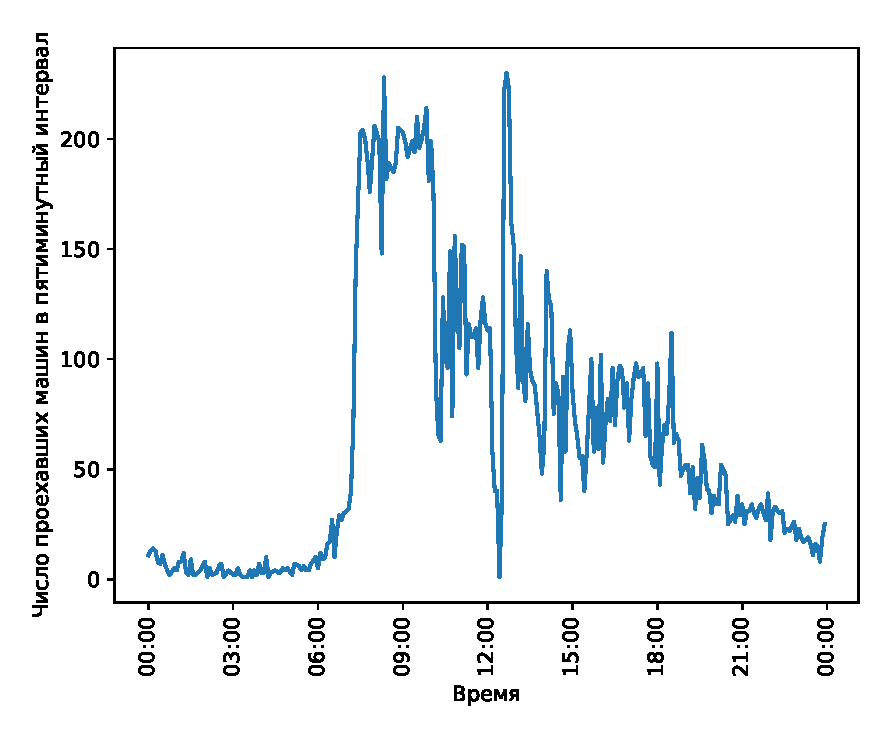
\includegraphics[width=0.6\linewidth]{Detector.eps}
    \caption{Данные с дорожного датчика за один день. Пиковая нагрузка 45 АТС/мин в 8:20.}
\end{figure}
\end{frame}

\begin{frame}
    \frametitle{Входной поток}
    \centering
    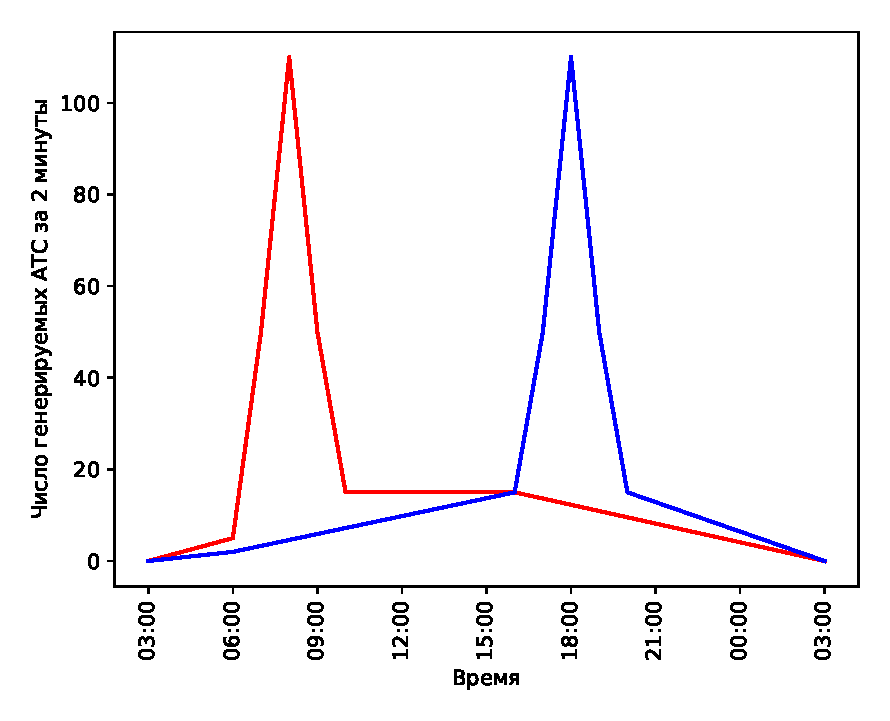
\includegraphics[width=0.75\linewidth]{MCAR_full_woenters_12_two_types_110_24h_3h_Enters_generators.eps} \\
    \hfill
    Графики загрузки двух типов въездов~--- с утренней и вечерней пиковыми загрузками
\end{frame}


\subsubsection{Обычные въезды}
\begin{frame}
    \frametitle{Число автомобилей на автомагистрали}
    \centering
    \begin{minipage}[b]{0.49\textwidth}
        \centering
        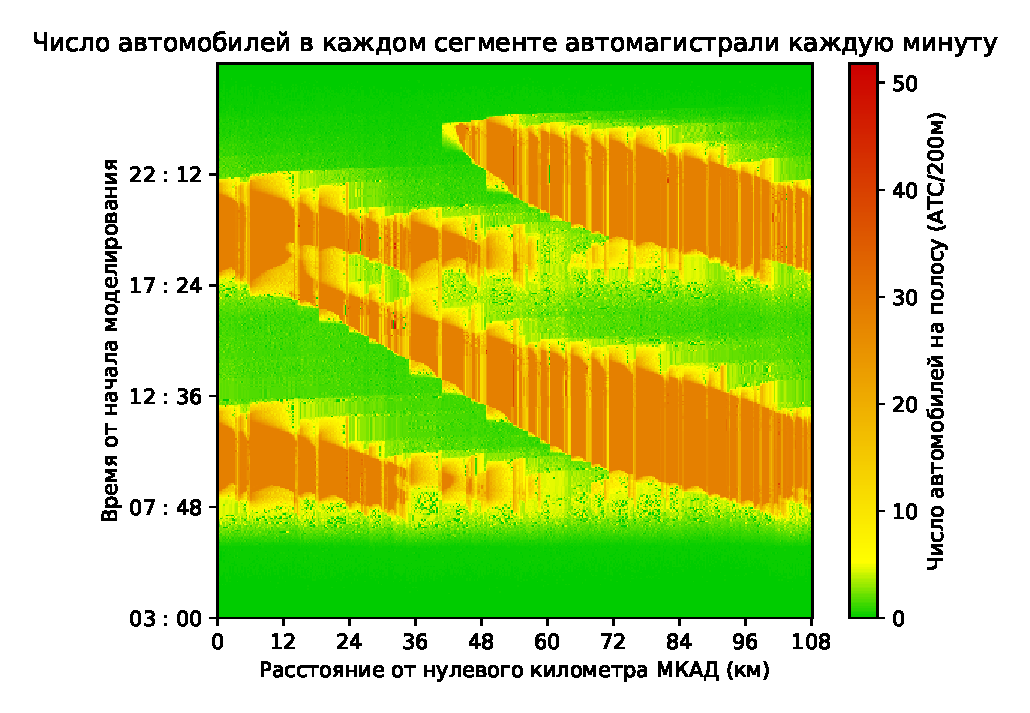
\includegraphics[width=1\linewidth]{MCAR_full_woenters_12_two_types_110_24h_3h.eps}  \\ а) Без управления въездами
    \end{minipage}
    \hfill
    \begin{minipage}[b]{0.49\textwidth}
        \centering
        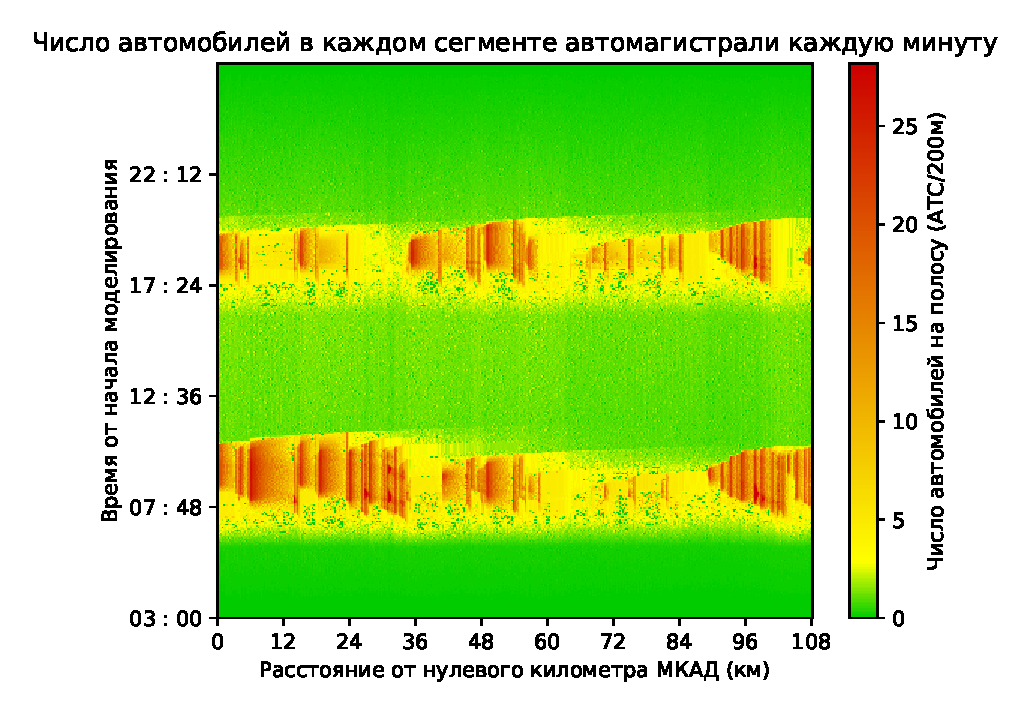
\includegraphics[width=1\linewidth]{MCAR_full_woenters_12_two_types_110_24h_3h_handcontrol.eps}  \\ b) С управлением въездами
    \end{minipage}
    \hfill
    Количество автомобилей на 200 метров в модели транспортной сети МКАД за день
\end{frame}


\begin{frame}
    \frametitle{Число въехавших автомобилей}
    \centering
    \begin{minipage}[b]{.49\textwidth}
        \centering
        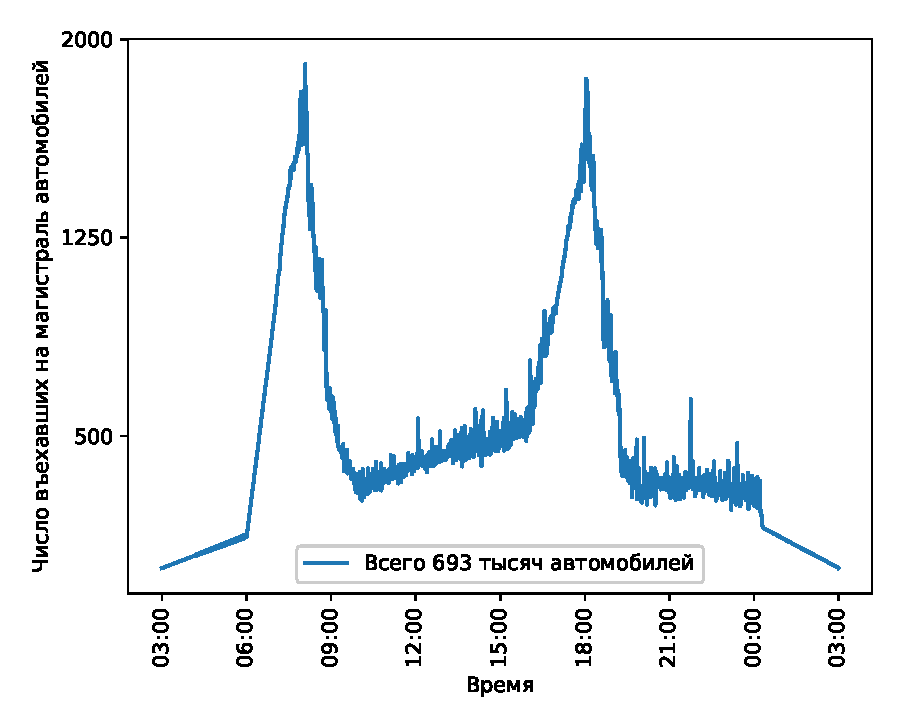
\includegraphics[width=1\linewidth]{MCAR_full_woenters_12_two_types_110_24h_3h_Entered.eps}  \\ а) Без управления въездами
    \end{minipage}
    \hfill
    \begin{minipage}[b]{.49\textwidth}
        \centering
        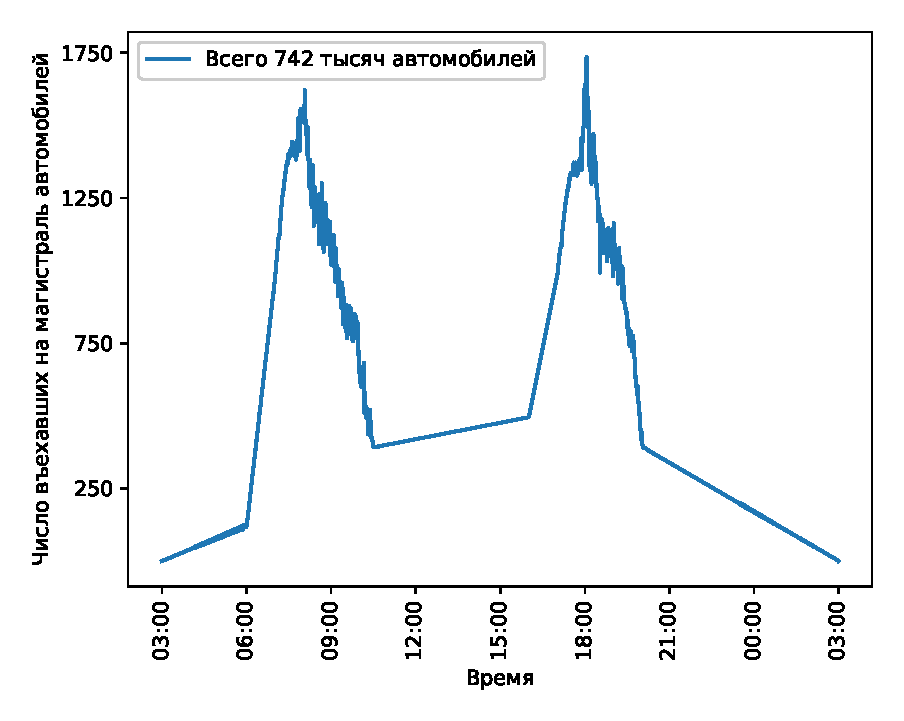
\includegraphics[width=1\linewidth]{MCAR_full_woenters_12_two_types_110_24h_3h_handcontrol_Entered.eps}  \\ b) С управлением въездами
    \end{minipage}
    \hfill
    Графики суммарно въехавшего на МКАД со всех въездов числа автомобилей
\end{frame}


\begin{frame}
    \frametitle{Временные потери на проезд по МКАД}
    \centering
    \begin{minipage}[b]{.49\textwidth}
        \centering
        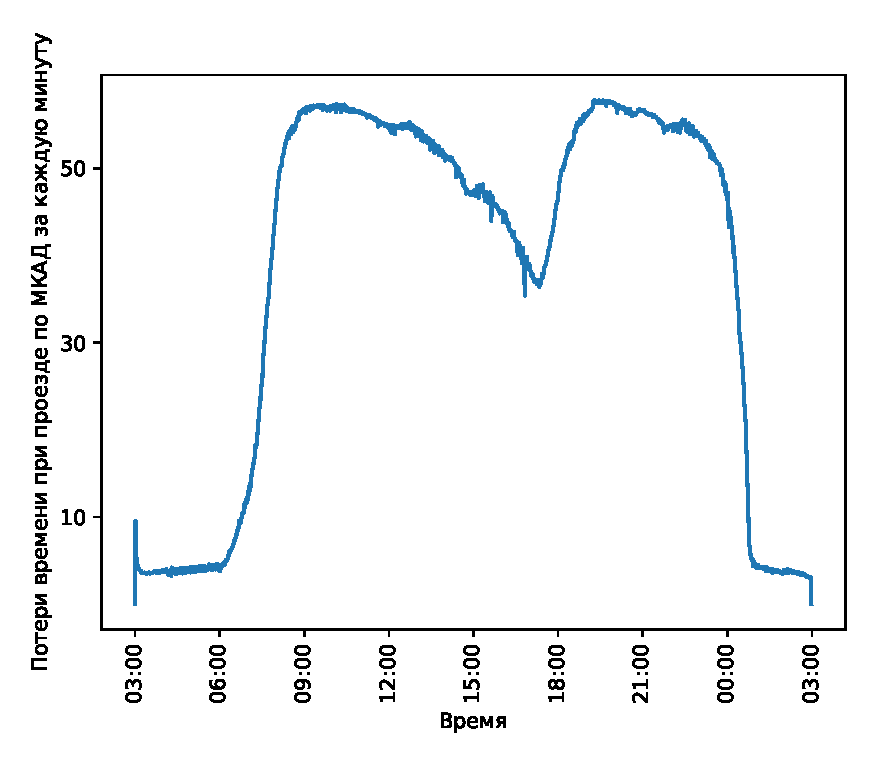
\includegraphics[width=1\linewidth]{MCAR_full_woenters_12_two_types_110_24h_3h_Time_to_pass.eps}  \\ а) Без управления въездами
    \end{minipage}
    \hfill
    \begin{minipage}[b]{.49\textwidth}
        \centering
        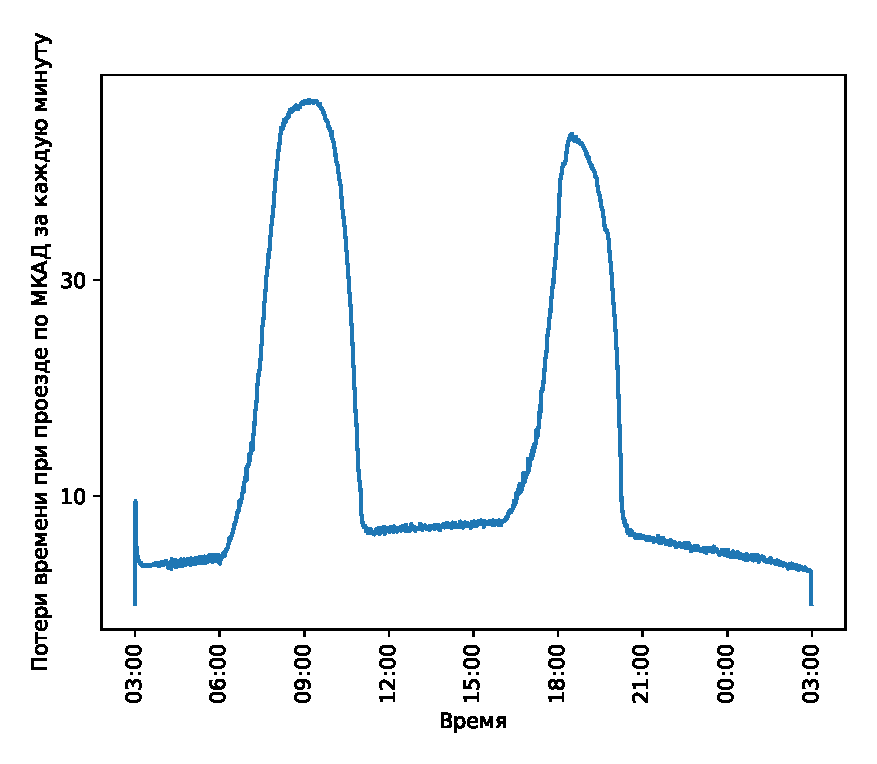
\includegraphics[width=1\linewidth]{MCAR_full_woenters_12_two_types_110_24h_3h_handcontrol_Time_to_pass.eps}  \\ b) С управлением въездами
    \end{minipage}
    \hfill
    Временные потери на проезд по МКАД относительно пустой автомагистрали
\end{frame}

\subsubsection{Длинные въезды}
\begin{frame}
    \frametitle{Число автомобилей на автомагистрали}
    \centering
    \begin{minipage}[b]{0.49\textwidth}
        \centering
        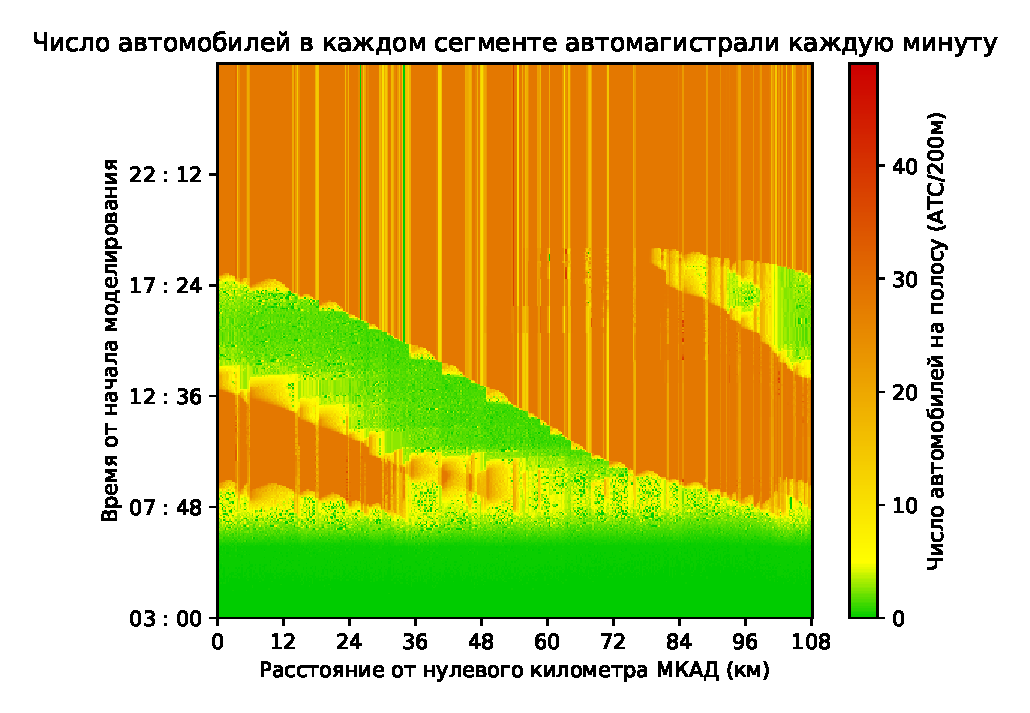
\includegraphics[width=1\linewidth]{MCAR_full_woenters_12_two_types_110_24h_3h_6km.eps}  \\ а) Без управления въездами
    \end{minipage}
    \hfill
    \begin{minipage}[b]{0.49\textwidth}
        \centering
        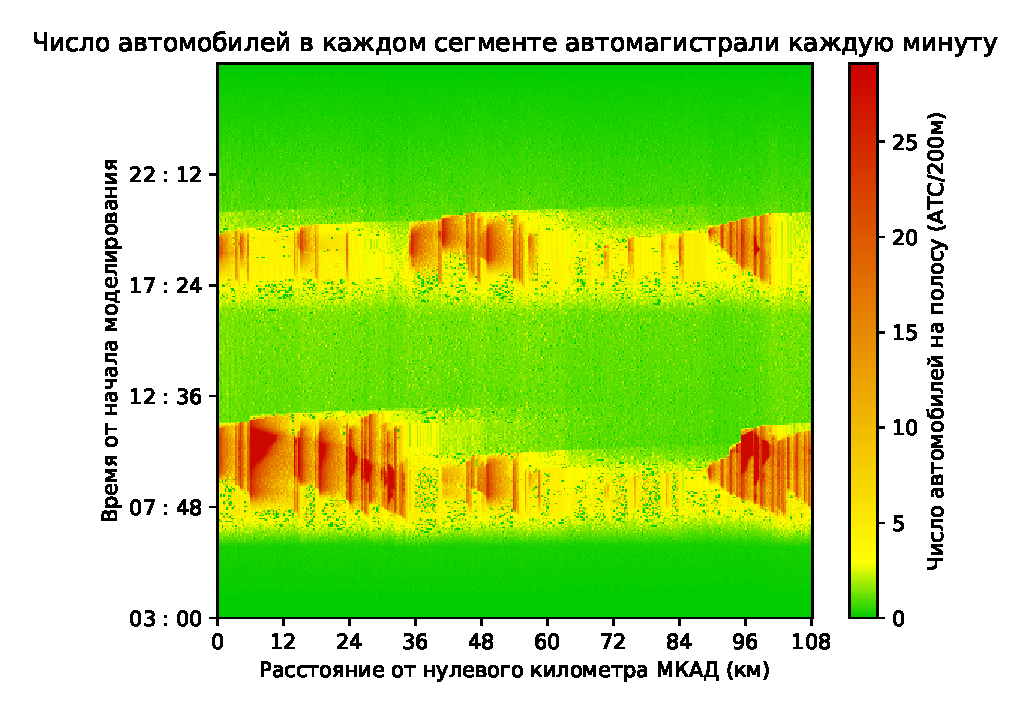
\includegraphics[width=1\linewidth]{MCAR_full_woenters_12_two_types_110_24h_3h_6km_handcontrol.eps}  \\ b) С управлением въездами
    \end{minipage}
    \hfill
    Количество автомобилей на 200 метров в модели транспортной сети МКАД за день
\end{frame}


\begin{frame}
    \frametitle{Число въехавших автомобилей}
    \centering
    \begin{minipage}[b]{.49\textwidth}
        \centering
        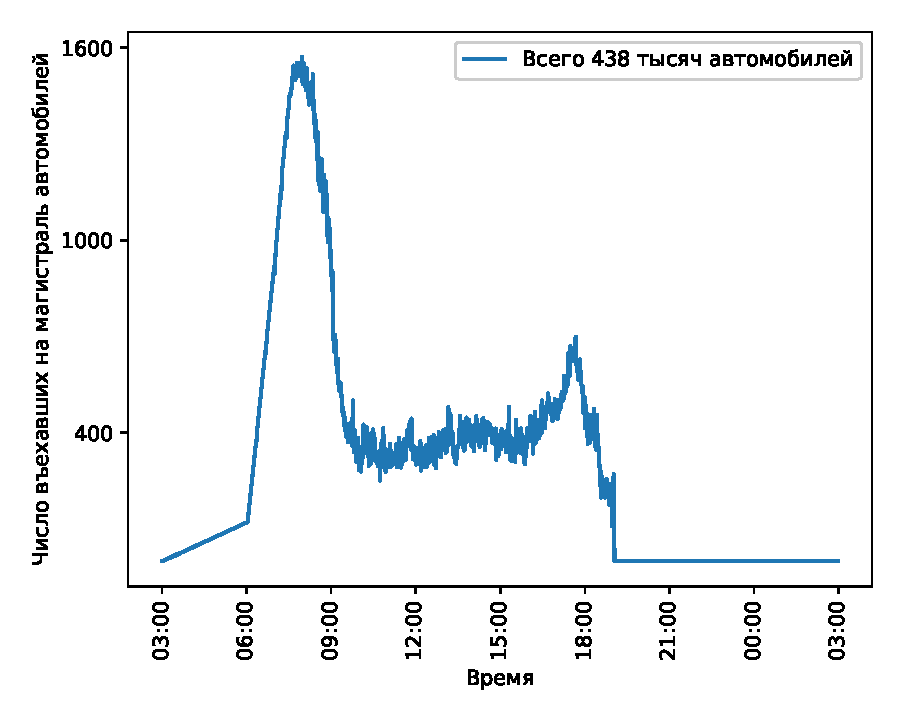
\includegraphics[width=1\linewidth]{MCAR_full_woenters_12_two_types_110_24h_3h_6km_Entered.eps}  \\ а) Без управления въездами
    \end{minipage}
    \hfill
    \begin{minipage}[b]{.49\textwidth}
        \centering
        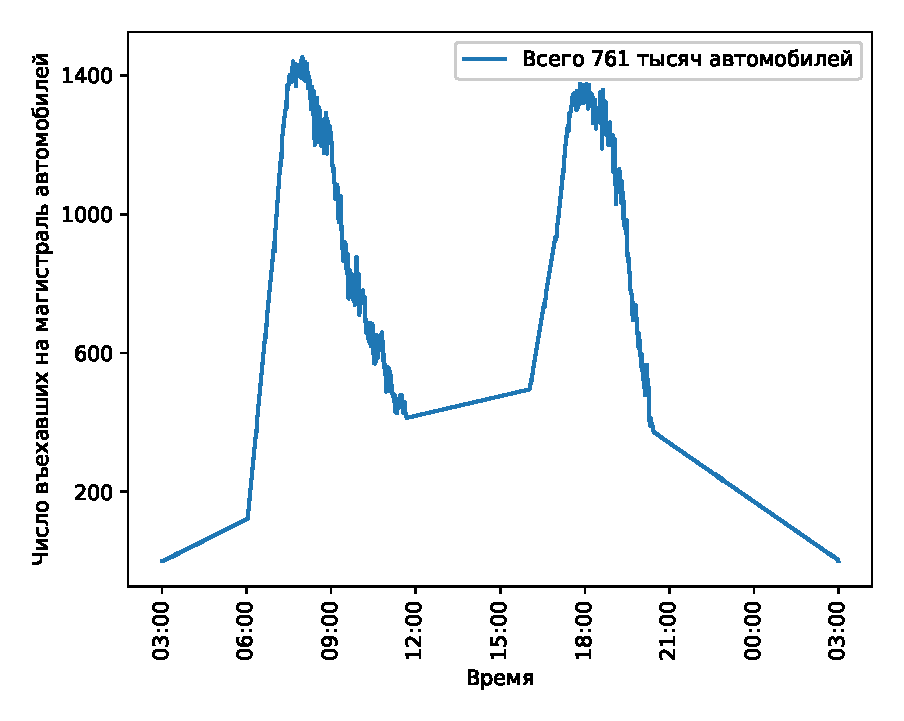
\includegraphics[width=1\linewidth]{MCAR_full_woenters_12_two_types_110_24h_3h_6km_handcontrol_Entered.eps}  \\ b) С управлением въездами
    \end{minipage}
    \hfill
    Графики суммарно въехавшего на МКАД со всех въездов числа автомобилей
\end{frame}


\begin{frame}
    \frametitle{Временные потери на проезд по МКАД}
    \centering
    \begin{minipage}[b]{.49\textwidth}
        \centering
        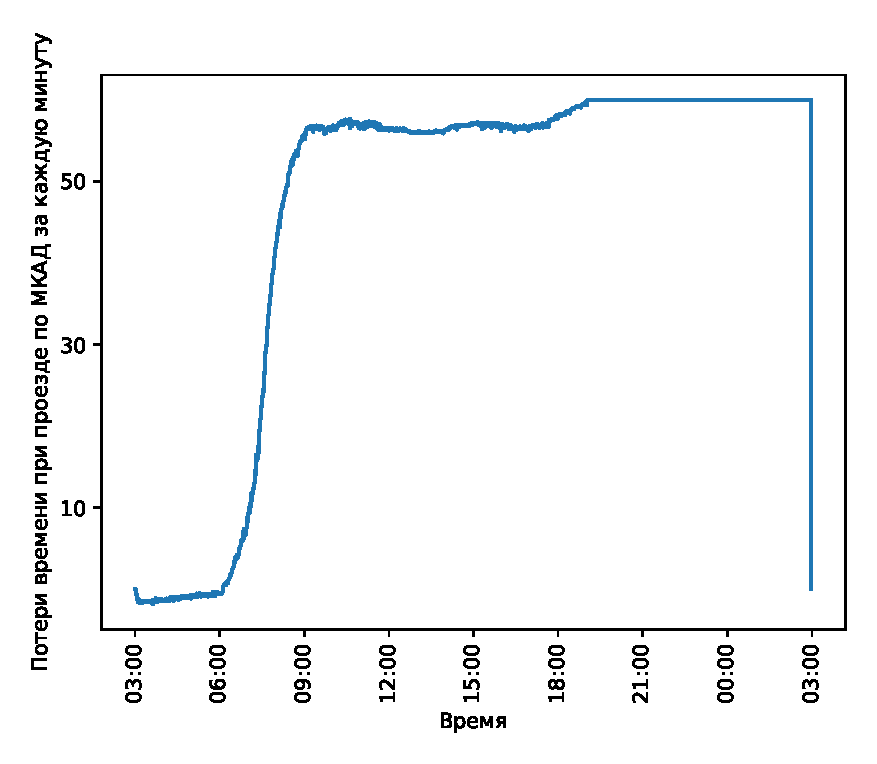
\includegraphics[width=1\linewidth]{MCAR_full_woenters_12_two_types_110_24h_3h_6km_Time_to_pass.eps}  \\ а) Без управления въездами
    \end{minipage}
    \hfill
    \begin{minipage}[b]{.49\textwidth}
        \centering
        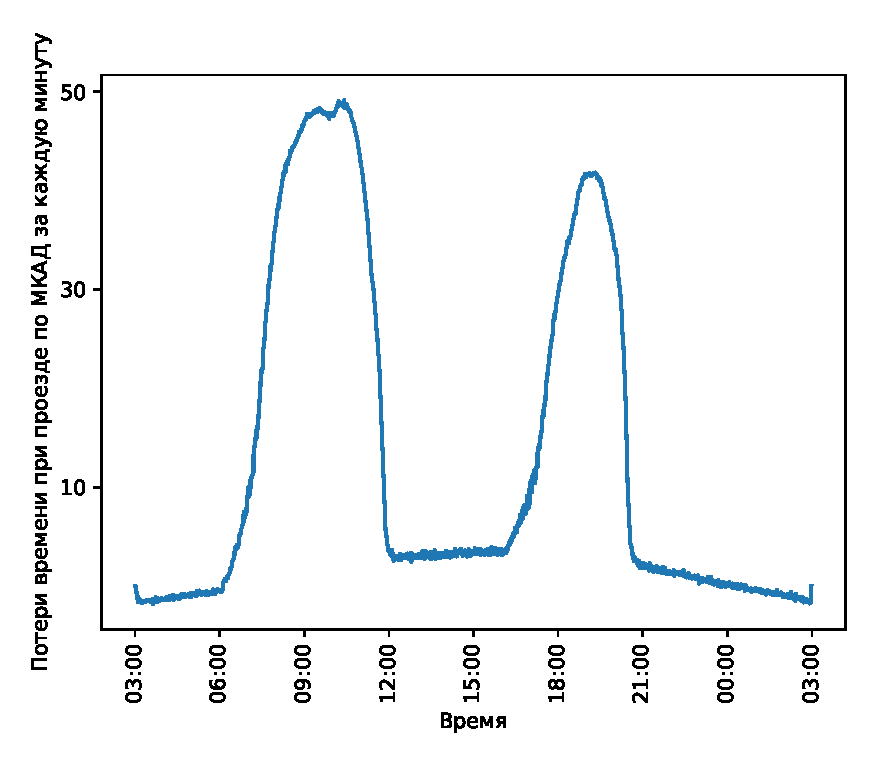
\includegraphics[width=1\linewidth]{MCAR_full_woenters_12_two_types_110_24h_3h_6km_handcontrol_Time_to_pass.eps}  \\ b) С управлением въездами
    \end{minipage}
    \hfill
    Временные потери на проезд по МКАД относительно пустой автомагистрали
\end{frame}


\subsection{Моделирование МКАД с вычислением всех фундаментальных диаграмм}
\begin{frame}[plain, noframenumbering]
    \begin{center}
        \Huge
        Моделирование МКАД с вычислением всех фундаментальных диаграмм
    \end{center}
\end{frame}
\begin{frame}
    \frametitle{Число автомобилей на автомагистрали}
    \centering
    \begin{minipage}[b]{0.49\textwidth}
        \centering
        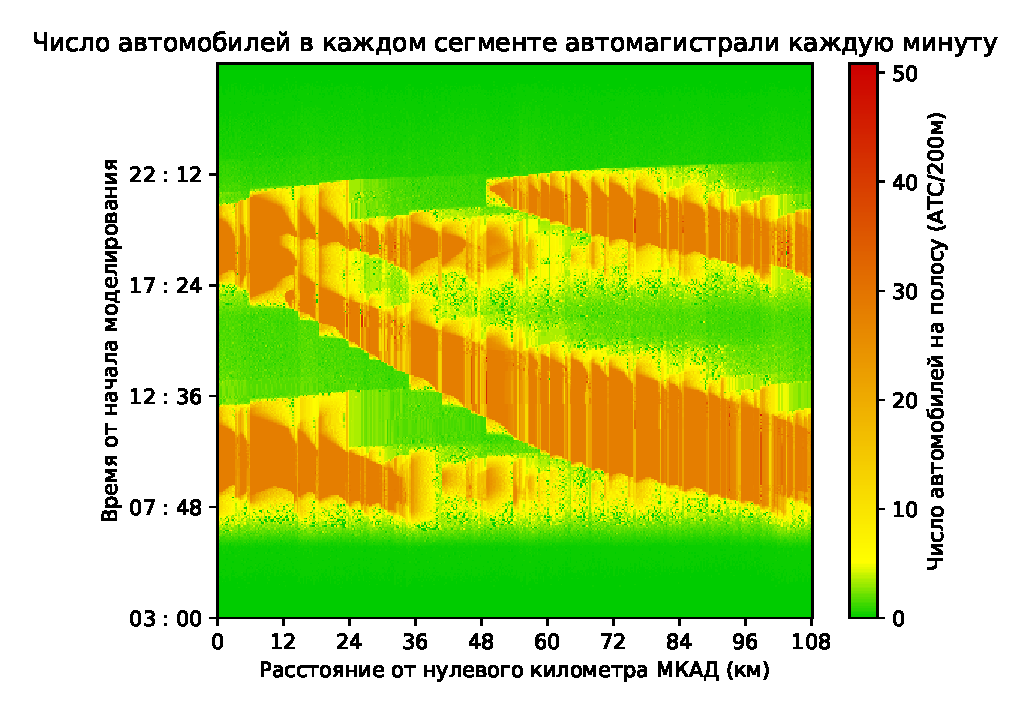
\includegraphics[width=1\linewidth]{MCAR_full_woenters_12_two_types_110_24h_3h_fullFD.eps}  \\ а) Без управления въездами
    \end{minipage}
    \hfill
    \begin{minipage}[b]{0.49\textwidth}
        \centering
        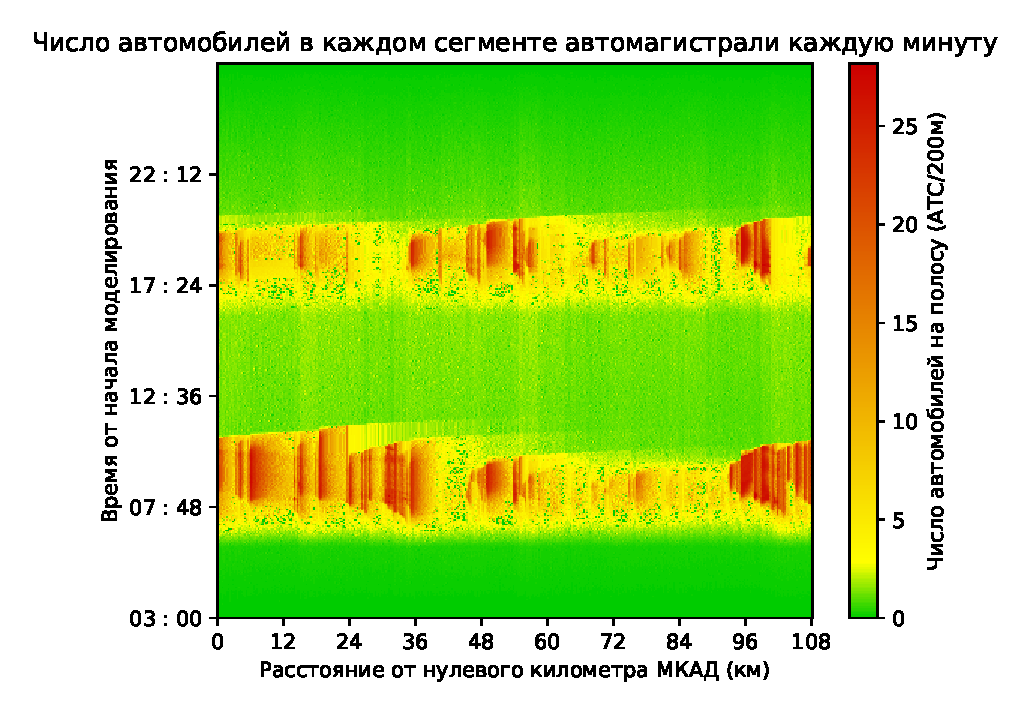
\includegraphics[width=1\linewidth]{MCAR_full_woenters_12_two_types_110_24h_3h_fullFD_handcontrol.eps}  \\ b) С управлением въездами
    \end{minipage}
    \hfill
    Количество автомобилей на 200 метров в модели транспортной сети МКАД за день
\end{frame}


\begin{frame}
    \frametitle{Число въехавших автомобилей}
    \centering
    \begin{minipage}[b]{.49\textwidth}
        \centering
        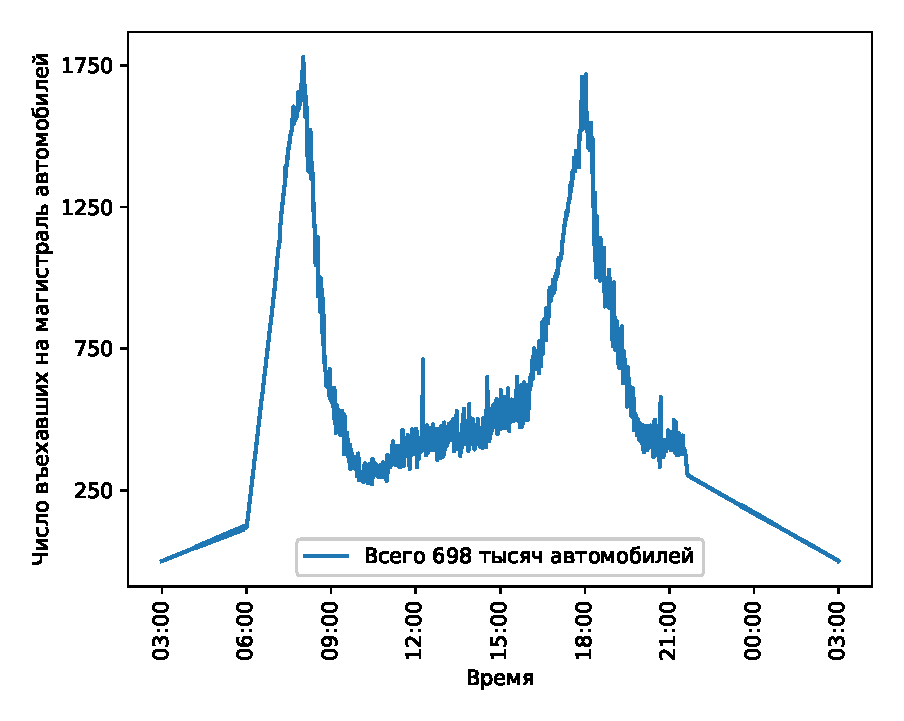
\includegraphics[width=1\linewidth]{MCAR_full_woenters_12_two_types_110_24h_3h_fullFD_Entered.eps}  \\ а) Без управления въездами
    \end{minipage}
    \hfill
    \begin{minipage}[b]{.49\textwidth}
        \centering
        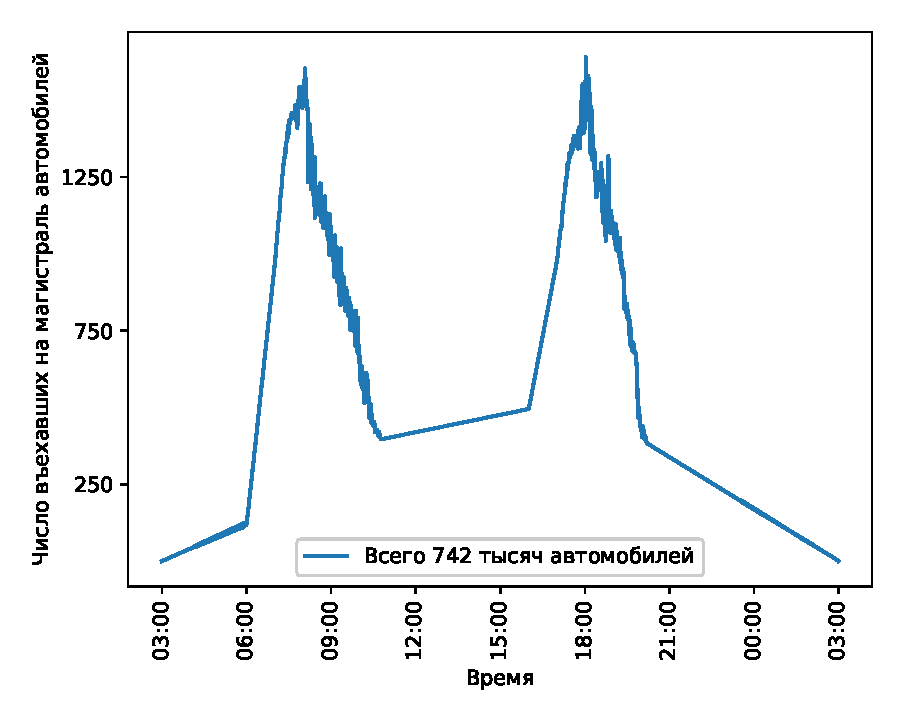
\includegraphics[width=1\linewidth]{MCAR_full_woenters_12_two_types_110_24h_3h_fullFD_handcontrol_Entered.eps}  \\ b) С управлением въездами
    \end{minipage}
    \hfill
    Графики суммарно въехавшего на МКАД со всех въездов числа автомобилей
\end{frame}


\begin{frame}
    \frametitle{Временные потери на проезд по МКАД}
    \centering
    \begin{minipage}[b]{.49\textwidth}
        \centering
        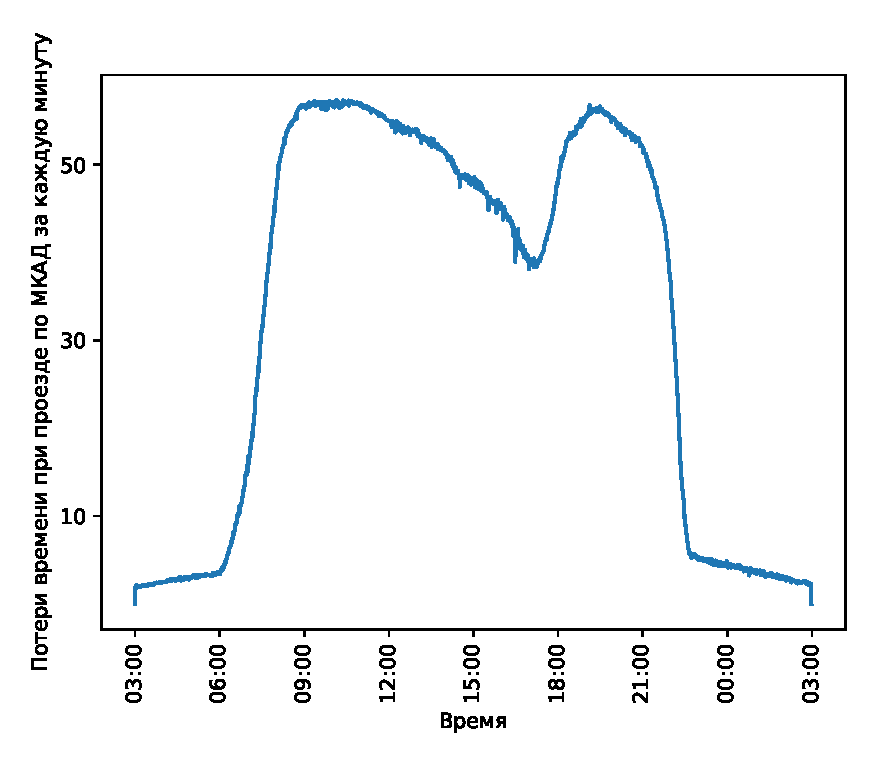
\includegraphics[width=1\linewidth]{MCAR_full_woenters_12_two_types_110_24h_3h_fullFD_Time_to_pass.eps}  \\ а) Без управления въездами
    \end{minipage}
    \hfill
    \begin{minipage}[b]{.49\textwidth}
        \centering
        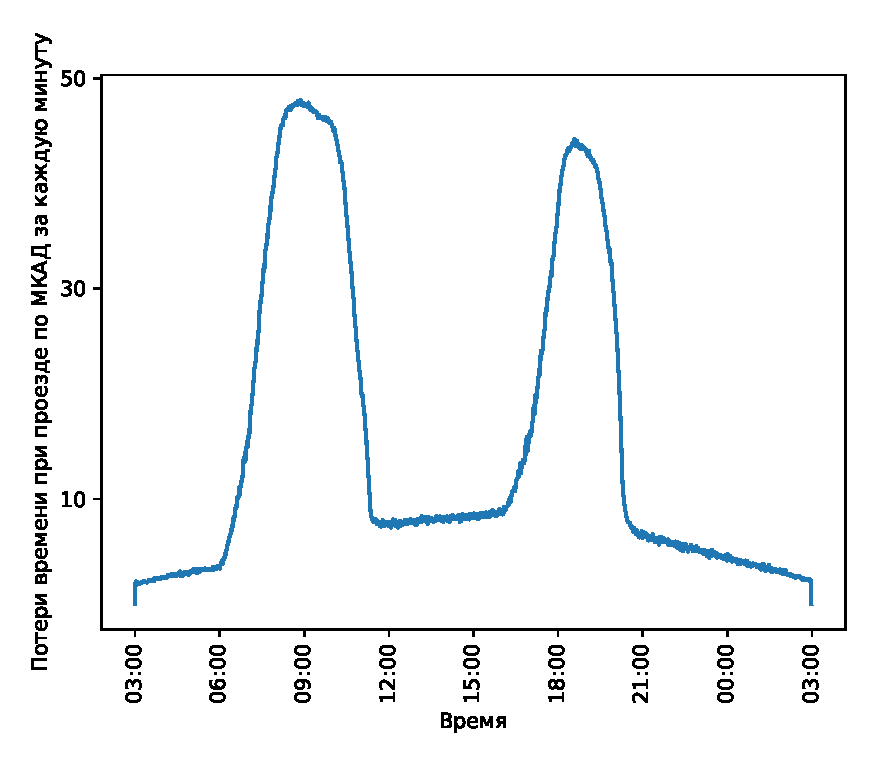
\includegraphics[width=1\linewidth]{MCAR_full_woenters_12_two_types_110_24h_3h_fullFD_handcontrol_Time_to_pass.eps}  \\ b) С управлением въездами
    \end{minipage}
    \hfill
    Временные потери на проезд по МКАД относительно пустой автомагистрали
\end{frame}


% [plain, noframenumbering]
